% A note of musixdoc.pdf
% Interpretter: XeTeX. XeTeX supports unicode. Guitar tablature and Chinese song lyrics in this article use wider unicode. Otherwise, the default interpretter of texmaker pdflatex is ok.
% A particular interpreting operation is required for this article, see the details in 1.3 The three pass system.  
\documentclass[11pt]{article}
%For A4 paper, portrait mode (210 mm × 297 mm)
%For letter-size paper, portrait mode (8.5 in × 11 in)

\usepackage[margin=1in]{geometry}

\usepackage{musixtex} % music score
\usepackage{graphicx}% insert graphs
\usepackage{amsmath} % to support numbered music notion

\usepackage{xeCJK} % Chinese for song lyrics
\setCJKfamilyfont{Ali}{Alibaba PuHuiTi} % Chinese font

% The LaTeX Font Catalogue, https://tug.org/FontCatalogue/
\usepackage[T1]{fontenc} % to set font of a word
%\usepackage{arev}% Font: https://tug.org/FontCatalogue/arev/

\usepackage{ipa} % phonetic notes

\usepackage{hyperref} % website link
\usepackage[none]{hyphenat}% Prevent LaTeX from using hyphenated words.

\usepackage{utfsym} % music symbole sharp\usym{266F} flat\usym{266D} natural\usym{266E}
\usepackage{textcomp} %  '\textquotesingle; ` \textasciigrave

\parindent 0ex % By default the paragraph is not indented, but the following paragraphes are indented. This removes the indent.

\title{\Huge\textbf{Reading MusiX\TeX\ Manual}}
\author{}

\begin{document}
\maketitle

This article is a note of the manual document of MusiX\TeX\cite{MusiXTeX}: \href{https://mirror.las.iastate.edu/tex-archive/macros/generic/musixtex/doc/musixdoc.pdf}{``MusiXTEX - Using TEX to write polyphonic or instrumental music"}.\\

The purposes are 1) to learning MusiX\TeX, 2) to write examples.\\

Sections are as numbered as the original document.

\section*{1 Introduction to MusiXTEX}
\subsection*{1.2 A simple example}
There is a framework for music scores. Referring to chapter 2, to define a framework, or in other words a \LaTeX\ ([\stress leitek], X is the Greek letter $\chi$ \cite{latextutorial}) music template, is to define Music size, Number of instruments, Instrument names, Number of staves per instrument, Key signatures, Clefs for each staff, Meters. \\

Basically, a music score is wrapped by the "music" markup in \LaTeX\ text.
\begin{verbatim}
\begin{music} 
% staffs 
\end{music}
\end{verbatim}

Within the "music" markup, we need to set up the framework of music sheet. For instance, is it a music score for a piano or for a guitar or for both? How many staves for each instrument? How to set the clef for each staff? What are the key signature, meter, tempo? And for staff layout itself, what's the size of the staff?\\

After that we start to write notes, the rhythm, the melody, the chords.\\

The basic staff line markup pair is \verb"\startextract" \verb"\endextract" \verb"\zendextract", or \verb"\startpiece" \verb"\endpiece" \verb"\zendpiece". The "extract" pair produce a part of a line and trims to the length of notes, it may exceed the paper width. The "piece" pair produce a line or multiple lines. "z" is a frequently used letter in command, another example \verb"\zw". I take it as the abbreviation of "zero". \verb"\zendpiece" zero bar, no end bar. \verb"\zw" to input a whole note with zero horizontal space so multiple whole note forms a chord. \\

No space line is allowed inside the \verb"\startpiece\endpiece" pair. Also empty is not allowed, otherwise the error is "Division by zero".\\

Then input notes by the command \verb"\notes ... \en". What are the markups for notes? How to input the C major scale with quarter notes? \verb"\notes \qa{cdefg'ab} \en". Why this way? Suppose one has these questions in mind while reading MusiX\TeX.\\

So if one uses the default setting of the MusiX\TeX\ framework, and input a "piece", we get a blank staff line with a Treble clef.\\
\begin{music} 
\startpiece
\notes\en
\zendpiece
\end{music}

The MusiX\TeX\ \LaTeX\ code is:\\
\begin{verbatim}
\documentclass{article}
\usepackage{musixtex}
\begin{document} 
\begin{music} 
\startpiece
\notes\en
\zendpiece
\end{music}
\end{document}
\end{verbatim}

Or input "extract", we get a head of the staff line.\\
\begin{music} 
\startextract
\notes\en
\endextract
\end{music}

\begin{verbatim}
\begin{music} 
\startextract
\notes\en
\endextract
\end{music}
\end{verbatim}

Or left aligned:\\
\begin{music} 
\let\extractline\leftline
\startextract
\notes\en
\endextract
\end{music}

\begin{verbatim}
\begin{music} 
\let\extractline\leftline
\startextract
\notes\en
\endextract
\end{music}
\end{verbatim}

Or a C major scale "piece":\\
\begin{music} 
\startpiece
\Notes \qa{cdefg'aba}\qa{!gfedc} \en
\zendpiece
\end{music}

\begin{verbatim}
\begin{music} 
\startpiece
\Notes \qa{cdefg'aba}\qa{!gfedc} \en
\zendpiece
\end{music}
\end{verbatim}

And C major scale "extract":\\
\begin{music} 
\let\extractline\leftline
\startextract
\Notes \qa{cdefg'aba}\qa{!gfedc} \en
\endextract
\end{music}

\begin{verbatim}
\begin{music} 
\let\extractline\leftline
\startextract
\Notes \qa{cdefg'aba}\qa{!gfedc} \en
\endextract
\end{music}
\end{verbatim}

And G major scale "extract":\\
\begin{music} 
\let\extractline\leftline
\startextract
\Notes \qa{g'abcde^fg^fedcba!g} \en
\endextract
\end{music}

\begin{verbatim}
\begin{music} 
\let\extractline\leftline
\startextract
\Notes \qa{g'abcde^fg^fedcba!g} \en
\endextract
\end{music}
\end{verbatim}

The document gives a real example of the two first bars of the sonata in C-major KV545 by Mozart.\\

\begin{music}
\normalmusicsize
\instrumentnumber{1} 
\parindent10mm % placeholder for the instrument name.
\setname1{Piano} 
\setstaffs1{2} 
\generalsignature{-3}
\generalmeter{\meterfrac44} % 4/4 meter chosen 
\startextract % starting real score
\Notes\ibu0f0\qb0{cge}\tbu0\qb0g|\hl j\en 
\Notes\ibu0f0\qb0{cge}\tbu0\qb0g|\ql l\sk\ql n\en
\bar
\Notes\ibu0f0\qb0{dgf}|\qlp i\en
\notes\tbu0\qb0g|\ibbl1j3\qb1j\tbl1\qb1k\en
\Notes\ibu0f0\qb0{cge}\tbu0\qb0g|\hl j\en
\zendextract % terminate excerpt without the end bar
\end{music}

\begin{verbatim}
\begin{music}
\normalmusicsize
\instrumentnumber{1} 
\parindent10mm % placeholder for the instrument name.
\setname1{Piano} 
\setstaffs1{2} 
\generalsignature{-3}
\generalmeter{\meterfrac44} % 4/4 meter chosen 
\startextract % starting real score
\Notes\ibu0f0\qb0{cge}\tbu0\qb0g|\hl j\en 
\Notes\ibu0f0\qb0{cge}\tbu0\qb0g|\ql l\sk\ql n\en
\bar
\Notes\ibu0f0\qb0{dgf}|\qlp i\en
\notes\tbu0\qb0g|\ibbl1j3\qb1j\tbl1\qb1k\en
\Notes\ibu0f0\qb0{cge}\tbu0\qb0g|\hl j\en
\zendextract % terminate excerpt without the end bar
\end{music}
\end{verbatim}

Let's see how to define a music sheet framework through the example.

\begin{itemize}
\item Music size\\
\verb"\smallmusicsize": 16pt-high staves\\
\verb"\normalmusicsize":20pt, default\\
\verb"\largemusicsize": 24pt\\
\verb"\Largemusicsize": 29pt

\item Number of instruments\\
\verb"\instrumentnumber{n}": n=1, 2,..,6. Default: 1. It is the total number of how many instruments.\\

Most of the commands in MusiX\TeX\ has a parameter of the instrument number, this is the label number \#i. For instance, if \verb"\instrumentnumber{3}", then there are at least 3 lines or groups of staves, one for each instrument. And the instruments are labeled \textbf{from the bottom} \#1, \#2, \#3. \\

Why from the bottom? The whole MusiX\TeX\ counts from the bottom, except Guitar tablature. It is similar with counting the staff lines, from the lowest, 1,2,3,4,5. Even writing the notes are organized from the bottom.\\

We can also set the instrument name. \verb"\setname{n}{name of the instrument}": This will place the name in the space to the left of the first staff or group of staves for instrument \#n. 
In the example,\verb"\setname1{Piano}". \\

\item Number of staves per instrument and staff group\\
\verb"\setstaffs{n}{p}": n is the label number \#n of the instrument. p is the number of staves. For example \verb"\setstaffs32" assigns two staves to the third instrument from the bottom. \\

And these 2 staves are grouped together with bars extending 2 staves.\\
In the example, \verb"\setstaffs1{2}".\\

\item Clefs\\
\verb"\setclef{n}{"$s_1s_2s_3s_4$\verb"}": n is the label number of the instrument \#n, $s_1$ is a digit specifying the clef for the first (lowest) staff, $s_2$ for the second staff, and so forth. \\
s=0, G clef, or \verb"\treble"\\
s=1 to 4, C-clef, 1 soprano, 3 alto \verb"\alto" and 4 tenor\\
s=5 to 7, F-clef, 5 baritone, 6 the normal bass \verb"\bass" \\
s=8 empty\\
s=9 a G clef on the first line, French violin clef\\

\verb"\bass \treble \alto" can be used instead of digits.\\

For example, a music sheet is for 2 instruments: a piano and a guitar. The piano is the \#2 instrument. So the staves are listed from the bottom: the 1st staff for the guitar, the above 2 staves for the piano. Now we need to set the clefs to the piano staff: \verb"\setclef{2}{\bass\treble}".\\

And two blank lines:\\
\begin{music}
\setclef18 
\nostartrule
\startpiece
\notes\en
\zendpiece
\end{music}
\begin{music}
\setclef18 
\nostartrule
\startpiece
\notes\en
\zendpiece
\end{music}
\begin{verbatim}
\begin{music}
\setclef18 
\nostartrule
\startpiece
\notes\en
\zendpiece
\end{music}
\begin{music}
\setclef18 
\nostartrule
\startpiece
\notes\en
\zendpiece
\end{music}
\end{verbatim}

\item Signature\\
\verb"\generalsignature{s}": where s > 0 is the number of sharps in the signature and s < 0 the number of flats. To override the common key signature for instrument n, use \verb"\setsign{n}{s}".\\

s is defined by the Circle of Fifths\cite{fifths} (see Figure \ref{fig:Fifths}), s=0 means C major or a minor, s=-2 is g minor or B\usym{266D}  major, s=3 is A major or f\usym{266F} minor, s=-1 means F major or d minor, s=1 means G major or e minor.
\verb"\generalsignature{-3}" is c minor or E\usym{266D} major.

\begin{figure}[ht!]% force here
\centering
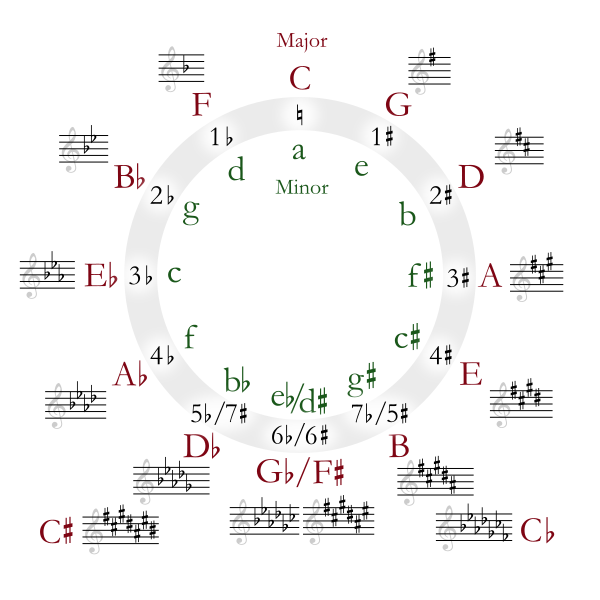
\includegraphics[width=3.3in]{Circle_of_Fifths}
\caption{The Circle of Fifths}
\label{fig:Fifths}
\end{figure}

\vspace{20pt}

\item meter\\
\verb"\generalmeter{\meterfrac44}" :% 4/4 meter chosen 

\item Tempo, or beats per minute. 
\verb"\metron{\qu}{60}" or \verb"\metronequiv{\qup}{\qu}": use \verb"\uptext{}" to place it in the beginning above the staff. Or text only, for example: \verb"Allegro cantabile", \verb"Larghetto maestoso".

\end{itemize}

\subsection*{1.3 The three pass system}
Like interpreting\cite{interpretter} external bibliography file is a sequence of operations, say xelatex + bibtex + xelatex + xelatex, there are three steps to compile a MusiX\TeX\ file.\footnote{At the beginning of the source code for TeX, Knuth calls TeX a "document compiler". But in The Art of Computer Programming, vol. 1, Knuth says that the TeX program is an interpreter for the TeX language, which produces output in DVI format, which can in turn be converted to PostScript, another interpreted language.--musarithmia}

\begin{verbatim}
xelatex filename
musixflx filename.mx1
xelatex filename
\end{verbatim}

Since there is no ``musixflx'' option in texmaker \textit{run} function, we need to manually input the commands in the Terminal window, say in a Macbook. \\

The reason is that \LaTeX\ writes the paper piece by piece like handwriting. Let's say it writes notes one by one on the staff. Then in the end \LaTeX\ finds the horizontal space between notes on one staff line should be adjusted aesthetically. So \LaTeX\ needs to rewrite the line. The output draft is filename.mx1. musixflx is to read it and to produce filename.mx2. \LaTeX\ rewrites the DVI file using both filename.mx1 and filename.mx2.\\

Please delete all temporary files first. In Terminal, switch to the file directory first\footnote{Switch to the file directory by inputting the command cd and pull the archive from Finder to show the directory.} and then execute 1st command and opening DVI file to see the rendering. Then the next command, and so on.

Please close the code window in texmaker. After the three-pass operation in Terminal, the code may not pass in texmaker with a red message: "energy stop" at a line \verb"\bar" or \verb"\contpiece". Then I delete the all temporary files again.

\subsubsection*{1.3.2 An example}
\begin{music}
\hsize=100mm
\generalmeter{\meterfrac24}%
\parindent 0pt
\generalsignature{-3}
\nostartrule
\startpiece\bigaccid
\NOtes\qu{ce}\en\bar
\NOtes\qu{gh}\en\bar
\NOtes\qu{=b}\en
\Notes\ds\cu g\en\bar
\NOtes\qu{^f=f}\en\bar
\NOtes\qu{=e}\itied0e\qu{_e}\en\bar
\Notes\ttie0\Qqbu ed{_d}c\en\bar
\Notes\ibu0b{-2}\qb0{=b}\en
\notes\nbbu0\qb0{=a}\tqh0N\en
\Notes\Dqbu cf\en\bar
\NOtes\uptext{\it tr}\qu e\uptext{\it tr}\qu d\en\bar
\NOtes\qu c\qp\en\mulooseness=1\Endpiece
\end{music}

\begin{verbatim}
\begin{music}
\hsize=100mm
\generalmeter{\meterfrac24}%
\parindent 0pt
\generalsignature{-3}
\nostartrule
\startpiece\bigaccid
\NOtes\qu{ce}\en\bar
\NOtes\qu{gh}\en\bar
\NOtes\qu{=b}\en
\Notes\ds\cu g\en\bar
\NOtes\qu{^f=f}\en\bar
\NOtes\qu{=e}\itied0e\qu{_e}\en\bar
\Notes\ttie0\Qqbu ed{_d}c\en\bar
\Notes\ibu0b{-2}\qb0{=b}\en
\notes\nbbu0\qb0{=a}\tqh0N\en
\Notes\Dqbu cf\en\bar
\NOtes\uptext{\it tr}\qu e\uptext{\it tr}\qu d\en\bar
\NOtes\qu c\qp\en\mulooseness=1\Endpiece
\end{music}
\end{verbatim}

If the very part of the PDF file doesn't look like the same, \textbf{3-pass interpretation} as said above. 

\subsection*{1.5 Installing and Using MusiXTEX}
I installed \LaTeX\ with the compiler Mac\TeX\ and the editor texmaker, following the \LaTeX\ tutorial by \href{https://www.michellekrummel.com/tutorials}{Ms. Michelle Krummel}\cite{latextutorial}. And MusiX\TeX\ is supported intrinsically.

\section*{4 Writing Notes}
\subsection*{4.1 Normal (unbeamed) spacing notes}
This is the method to input notes: 

%Verbatim allows us to write the text as we write it, this is, like if it were plain text. We can use verbatim in-text or in several lines. For in-line text, we need to use \verb and to set its scope we can use " ", ! !, ’ ’, @ @ these are to set its scope, any of them have the same function.
\begin{verbatim}
\notes...\en
\end{verbatim}

It is the characteristic word of MusiX\TeX.\\

\verb'\Notes' or \verb'\NOtes' or more capital letters means more horizontal space for the note.\\

\verb'\notes...|...\en' the absolute value mark is used to switch to another staff, e.g. as for piano staves to switch from the bass staff to the treble one, bar by bar in perfect synchronization. The designers said music ``has the form of a two-dimensional matrix". \\

\verb'\notes...|...&...\en' the ampersand mark means to switch to another instrument.\\ 

For \verb'\notes ... % ...\en', the percent mark \verb'%' is to separate the line for code writing convenience for the line is too long, though a bit confusing because \LaTeX\ uses \verb'%' for comments in coding. For example:\\

\begin{music}
\let\extractline\leftline
\startextract
\NOtes\lpar g\rpar g\hu g\sk%
\loffset{1.5}{\lpar g\rpar g}\loffset{.4}{\sh g}\hu g\sk%
\loffset{2.1}{\lpar g}\loffset{1.5}{\rpar g}\loffset{.4}{\dfl g}\hu g\en
\endextract
\end{music}
\begin{verbatim} 
\begin{music}
\let\extractline\leftline
\startextract
\NOtes\lpar g\rpar g\hu g\sk%
\loffset{1.5}{\lpar g\rpar g}\loffset{.4}{\sh g}\hu g\sk%
\loffset{2.1}{\lpar g}\loffset{1.5}{\rpar g}\loffset{.4}{\dfl g}\hu g\en
\endextract
\end{music}
\end{verbatim}

\verb"\wh" a whole note.\\

\verb"\hu" a half note with the stem going up; \verb"\hl" a half note with a stem going down on the left; \verb"\ha"  a half note with a stem automatically set by default: if the notehead of a music note is on the third line of the staff or above, the stems go down on the left. Otherwise, the stem goes up on the right. \\

\verb"\qu" a quarter note with a upward stem.\\

\verb"\cqu" a eighth note with a upward stem. The “c” within this macro name stands for the equivalent British term “crotchet” since the eighth note has a flag on the stem, it looks like a crotchet.\\

\verb"\lpar \rpar" is the left and right parentheses.\\

\verb"\loffset{N}{} or \roffset{N}{}" is left or right offset, where N is the distance to be shifted in note head widths. \\

\textquotesingle\ before a note means to transpose the note an octave higher and \textasciigrave before a note means an octave lower. And the transposition lasts the following notes inside the place holders  \verb"\notes" \verb"xxx" \verb"& yyy" \verb"| zzz \en". We can transpose the note explicitly using \verb"\transpose=n". We can also resume the pitch by put ! in front of a pitch, or set \verb"\transpose=\normaltranspose". \\

For example chord C7 in C major is C E G B\usym{266D}. The interval pattern is (4 3 3), i.e. the distance from C to E is 4 semitones, E to G 3 semitones, and G to B\usym{266D} is 3 semitones. \\

E major scale: E F\usym{266F} G\usym{266F} A B C\usym{266F} D\usym{266F}. E7 should be E G\usym{266F} B D. The signature of E major is 4 sharp signature because there are 4 sharps in the E major scale, but when we read the sheet, there should be 6 sharps in the treble staff, because the 1st space is F\usym{266F} and the 2nd line is G\usym{266F} as well. And of course there are also invisible sharps in ledger lines whenever its pitch name is FGCD (see the 1st bar).\\

One can use \verb"\transpose=2" to compose a E7 from C7 (see bar 2).\\

The E\usym{266D} major scale is E\usym{266D} F G A\usym{266D} B\usym{266D} C D. There are 3 flats in the key signature. But we can make a E\usym{266D}7 by transposing a C7  (see bar 2).\\


\begin{music}
\let\extractline\leftline
\nostartrule% no start bar
%\nobarnumbers % no bar numbering
\generalsignature{0}% C major
\parindent0pt
\startextract
% bar 1
\notes \zchar{15}{\scriptsize C major}\en % Key signature
\NOTEs \zchar{10}{\tiny C7}\zw{ceg'_b}\en

% bar 2
\generalsignature{4}% E major: E F# G# A B C# D# E
\ignorenats\Changecontext
\NOTEs \zchar{15}{\scriptsize E major}\en % Key signature
\notes \sh{f}\zchar{-0.1}{\tiny F}\en
\notes \sh{g}\zchar{1}{\tiny G}\en
\notes \sh{'c}\zchar{4}{\tiny C}\en
\notes \sh{'d}\zchar{5.2}{\tiny D}\en
\notes \loffset{8}{\sh{'f}\zchar{6.7}{\tiny F}}\en
\notes \loffset{8}{\sh{'g}\zchar{8}{\tiny G}}\en
\NOTEs  \zchar{9}{\tiny E7}\transpose=2\lsh{'b}\zw{`ceg'_b}\en
\NOTEs \roffset{1}{\zchar{10}{\tiny E7}\zw{eg'b=d}}\en

% bar 3
\setsign{1}{-3} %Eb mojor: Eb F G Ab Bb C D Eb
\ignorenats\Changecontext%
\Notes \zchar{15}{\scriptsize E\usym{266D} major}\en
\NOTEs \zchar{9}{\tiny E\usym{266D}7}\transpose=2\zw{ceg'_b}\en
\NOTEs \roffset{1}{\zchar{9}{\tiny E\usym{266D}7}\zw{eg'b_d}}\en
\zendextract
\end{music}

\begin{verbatim}
\begin{music}
\let\extractline\leftline
\nostartrule% no start bar
%\nobarnumbers % no bar numbering
\generalsignature{0}% C major
\parindent0pt
\startextract
% bar 1
\notes \zchar{15}{\scriptsize C major}\en % Key signature
\NOTEs \zchar{10}{\tiny C7}\zw{ceg'_b}\en

% bar 2
\generalsignature{4}% E major: E F# G# A B C# D# E
\ignorenats\Changecontext
\NOTEs \zchar{15}{\scriptsize E major}\en % Key signature
\notes \sh{f}\zchar{-0.1}{\tiny F}\en
\notes \sh{g}\zchar{1}{\tiny G}\en
\notes \sh{'c}\zchar{4}{\tiny C}\en
\notes \sh{'d}\zchar{5.2}{\tiny D}\en
\notes \loffset{8}{\sh{'f}\zchar{6.7}{\tiny F}}\en
\notes \loffset{8}{\sh{'g}\zchar{8}{\tiny G}}\en
\NOTEs  \zchar{9}{\tiny E7}\transpose=2\lsh{'b}\zw{`ceg'_b}\en
\NOTEs \roffset{1}{\zchar{10}{\tiny E7}\zw{eg'b=d}}\en

% bar 3
\setsign{1}{-3} %Eb mojor: Eb F G Ab Bb C D Eb
\ignorenats\Changecontext%
\Notes \zchar{15}{\scriptsize E\usym{266D} major}\en
\NOTEs \zchar{9}{\tiny E\usym{266D}7}\transpose=2\zw{ceg'_b}\en
\NOTEs \roffset{1}{\zchar{9}{\tiny E\usym{266D}7}\zw{eg'b_d}}\en
\zendextract
\end{music}
\end{verbatim}

\vspace{20pt}

Let's look at minor scales.\\

c minor scale: C D E\usym{266D} F G A\usym{266D} B\usym{266D} C. In fact, c minor scale and E\usym{266D} major scale share the signature of 3 flats. The interval pattern of Chord Cm7 is (3 4 3), so Chord Cm7 is C E\usym{266D} G B\usym{266D}. With the preceding flats in signature, we can still transpose Cm7 in C major to form a Cm7 in c minor scale (see bar 2). 

We can also transpose a Cm7 in c minor scale to form a Fm7 in f minor scale (see bar 3) and in c\usym{266F} minor scale (see bar 4).

I hope that sharps flats and naturals are one space high to align with the note head which is space height big \verb"Interligne". No, a little bit smaller than the space height so flats or sharps in a row don't touch each other.\\

\begin{music}
\let\extractline\leftline
\nostartrule% no start bar
%\nobarnumbers % no bar numbering 
\smallmusicsize
\generalsignature{0} % C major
\parindent0pt

\startextract
% bar 1
\notes \zchar{15}{\scriptsize C major}\en % Key signature
\NOTEs \zchar{10}{\tiny Cm7}\zw{c_eg'_b}\en

% bar 2
\generalsignature{-3}\ignorenats\Changecontext
% c minor: C D Eb F G Ab Bb C
\notes \zchar{15}{\scriptsize c minor}\en % Key signature
\scale{1.2}\NOTEs \zchar{10}{\tiny Cm7}\zw{ceg'b}\en\scale{1}

% bar 3
\setsign{1}{-3} %f minor: F G Ab Bb C Db Eb F
\ignorenats\Changecontext%
\scale{1.5}\NOTEs \zchar{15}{\scriptsize f minor}\roffset{1}%
{\zchar{10}{\tiny Fm7}\zw{f'ace}}\en\scale{1}

% bar 4
\generalsignature{4}% c# minor (E major): C# D# E F# G# A B C#
\ignorenats\Changecontext
\scale{1.5}\NOTEs \zchar{15}{\scriptsize c\usym{266F} minor}%
\zchar{10}{\tiny C\usym{266F}m7}\zw{ceg'b}\en\scale{1}
\zendextract
\end{music}

\begin{verbatim}
\begin{music}
\let\extractline\leftline
\nostartrule% no start bar
%\nobarnumbers % no bar numbering 
\smallmusicsize
\generalsignature{0} % C major
\parindent0pt
\startextract
% bar 1
\notes \zchar{15}{\scriptsize C major}\en % Key signature
\NOTEs \zchar{10}{\tiny Cm7}\zw{c_eg'_b}\en

% bar 2
\generalsignature{-3}\ignorenats\Changecontext
% c minor: C D Eb F G Ab Bb C
\notes \zchar{15}{\scriptsize c minor}\en % Key signature
\NOTEs \zchar{10}{\tiny Cm7}\zw{ceg'b}\en

% bar 3
\setsign{1}{-3} %f minor: F G Ab Bb C Db Eb F
\ignorenats\Changecontext%
\NOTEs \zchar{15}{\scriptsize f minor}\roffset{1}%
{\zchar{10}{\tiny Fm7}\zw{f'ace}}\en

% bar 4
\generalsignature{4}% c# minor (E major): C# D# E F# G# A B C#
\ignorenats\Changecontext
\NOTEs \zchar{15}{\scriptsize c\usym{266F} minor}%
\zchar{10}{\tiny C\usym{266F}m7}\zw{ceg'b}\en
\zendextract
\end{music}
\end{verbatim}

\vspace{20pt}

\textasciicircum\ before a note means sharp, a semitone higher, and \verb"_" before a note means flat, a semitone lower, = means a natural symbol before a note.  But accidental symbols might be overlaps, so \verb"\lsh{p}" or \verb"\lfl{p}" or even \verb"\loffset"are used to left shift the accidentals. The width of the accidentals of sharp, flat and natural might be 0.8 note head width.

Notes or chords\cite{allchords, inversion} or some symbols are listed below {Plese see the MusiX\TeX\ commands in \textbf{Appendix}}.

\vspace{20pt}
\textbf{Pitches}
\vspace{20pt}

Pitches defined by the frequency of the instrument are labeled as letter CDEFGAB and their lower-case letters and letters with prefixes. They are mapping to the spaces and lines of the staff one-to-one. \\

The document says: ``\verb@\wh a@ produces a whole note at nominal frequency 222.5 Hz'', ``\verb@\qu c@ produces an up-stemmed quarter note C (250 Hz)''. \\

We usually sing the numbered music notations, there are Fixed Do[d\schwa u] solf\`ege and movable Do solf\`ege. Let's say the numbered music notation here are Fixed Do solf\`ege or movable Do solf\`ege in C major scale.\\

% bass notes
\begin{music}
\let\extractline\leftline
\smallmusicsize
\instrumentnumber{1} % a single instrument
\setclef1{\bass}
\nostartrule
\parindent0pt
\startextract
%\Notes \wh{`ABCDEFG} \en % Not tokens
%\Notes \wh{`A} \wh{BCDEFG} \en % The transposition holds inside the \Notes...\en pair. 
\Notes \loffset{1}{\zchar{16}{\scriptsize \textasciigrave A}}%
\zchar{12}{\scriptsize $\underset{\dot{\dot{\dot{\dot{}}}}}6$}\wh{`A}\en

\Notes \loffset{1}{\zchar{16}{\scriptsize \textasciigrave B}}%
\zchar{12}{\scriptsize $\underset{\dot{\dot{\dot{\dot{}}}}}7$}\wh{`B}\en

\Notes \loffset{1}{\zchar{16}{\scriptsize \textasciigrave C}}%
\zchar{12}{\scriptsize $\underset{\dot{\dot{\dot{}}}}1$}\wh{`C}\en

\Notes \loffset{1}{\zchar{16}{\scriptsize \textasciigrave D}}%
\zchar{12}{\scriptsize $\underset{\dot{\dot{\dot{}}}}2$}\wh{`D}\en

\Notes \loffset{1}{\zchar{16}{\scriptsize \textasciigrave E}}%
\zchar{12}{\scriptsize $\underset{\dot{\dot{\dot{}}}}3$}\wh{`E}\en

\Notes \loffset{1}{\zchar{16}{\scriptsize \textasciigrave F}}%
\zchar{12}{\scriptsize $\underset{\dot{\dot{\dot{}}}}4$}\wh{`F}\en

\Notes \loffset{1}{\zchar{16}{\scriptsize \textasciigrave G}}%
\zchar{12}{\scriptsize $\underset{\dot{\dot{\dot{}}}}5$}\wh{`G}\en  

\Notes \zchar{16}{\scriptsize A}% 
\zchar{12}{\scriptsize $\underset{\dot{\dot{\dot{}}}}6$}\wh{A}\en

\Notes \zchar{16}{\scriptsize B}%
\zchar{12}{\scriptsize $\underset{\dot{\dot{\dot{}}}}7$}\wh{B}\en

\Notes \zchar{16}{\scriptsize C}%
\zchar{12}{\scriptsize $\underset{\dot{\dot{}}}1$}\wh{C}\en

\Notes \zchar{16}{\scriptsize D}%
\zchar{12}{\scriptsize $\underset{\dot{\dot{}}}2$}\wh{D}\en

\Notes \zchar{16}{\scriptsize E}% 
\zchar{12}{\scriptsize $\underset{\dot{\dot{}}}3$}\wh{E}\en

\Notes \zchar{16}{\scriptsize F}%
\zchar{12}{\scriptsize $\underset{\dot{\dot{}}}4$}\wh{F}\en

\Notes \zchar{16}{\scriptsize G}% 
\zchar{12}{\scriptsize $\underset{\dot{\dot{}}}5$}\wh{G}\en 

\Notes \loffset{1}{\zchar{16}{\scriptsize \textasciigrave a}}%
\zchar{12}{\scriptsize $\underset{\dot{\dot{}}}6$}\wh{`a}\en

\Notes \loffset{1}{\zchar{16}{\scriptsize \textasciigrave b}}%
\zchar{12}{\scriptsize $\underset{\dot{\dot{}}}7$}\wh{`b}\en

\Notes \loffset{1}{\zchar{16}{\scriptsize \textasciigrave c}}%
\zchar{12}{\scriptsize $\underset{\dot{}}1$}\wh{`c}\en

\Notes \loffset{1}{\zchar{16}{\scriptsize \textasciigrave d}}%
\zchar{12}{\scriptsize $\underset{\dot{}}2$}\wh{`d}\en

\Notes \loffset{1}{\zchar{16}{\scriptsize \textasciigrave e}}%
\zchar{12}{\scriptsize $\underset{\dot{}}3$}\wh{`e}\en

\Notes \loffset{0.5}{\zchar{16}{\scriptsize \textasciigrave f}}%
\zchar{12}{\scriptsize $\underset{\dot{}}4$}\wh{`f}\en

\Notes \zchar{16}{\scriptsize \textasciigrave g}
\zchar{12}{\scriptsize $\underset{\dot{}}5$}\wh{`g}\en 
%`a = 'A = H,`b ='B = I,`c = 'C = J,`d = 'D = K,
%`e = 'E = L,`f = 'F = M,`g = 'G = N
\Notes \zchar{16}{\scriptsize a}%
\zchar{12}{\scriptsize $\underset{\dot{}}6$}\wh{a}\en

\Notes \zchar{16}{\scriptsize b}%
\zchar{12}{\scriptsize $\underset{\dot{}}7$}\wh{b}\en

\Notes \zchar{16}{\scriptsize c}%
\zchar{12}{\scriptsize $1$}\wh{c}\en% middle C

\zendextract 
\end{music}
%\let\extractline\leftline
%\smallmusicsize
%\instrumentnumber{1} % a single instrument
%\setclef1{\bass}
%\nostartrule
%\parindent0pt
%\startextract
%%\Notes \wh{`ABCDEFG} \en % Not tokens
%% \Notes \wh{`A} \wh{BCDEFG} \en % The transposition holds inside 
%% the \Notes...\en pair. 
%\Notes \loffset{1}{\zchar{16}{\scriptsize \textasciigrave A}}%
%\zchar{12}{\scriptsize $\underset{\dot{\dot{\dot{\dot{}}}}}6$}\wh{`A}\en
%
%\Notes \loffset{1}{\zchar{16}{\scriptsize \textasciigrave B}}%
%\zchar{12}{\scriptsize $\underset{\dot{\dot{\dot{\dot{}}}}}7$}\wh{`B}\en
%
%\Notes \loffset{1}{\zchar{16}{\scriptsize \textasciigrave C}}%
%\zchar{12}{\scriptsize $\underset{\dot{\dot{\dot{}}}}1$}\wh{`C}\en
%
%\Notes \loffset{1}{\zchar{16}{\scriptsize \textasciigrave D}}%
%\zchar{12}{\scriptsize $\underset{\dot{\dot{\dot{}}}}2$}\wh{`D}\en
%
%\Notes \loffset{1}{\zchar{16}{\scriptsize \textasciigrave E}}%
%\zchar{12}{\scriptsize $\underset{\dot{\dot{\dot{}}}}3$}\wh{`E}\en
%
%\Notes \loffset{1}{\zchar{16}{\scriptsize \textasciigrave F}}%
%\zchar{12}{\scriptsize $\underset{\dot{\dot{\dot{}}}}4$}\wh{`F}\en
%
%\Notes \loffset{1}{\zchar{16}{\scriptsize \textasciigrave G}}%
%\zchar{12}{\scriptsize $\underset{\dot{\dot{\dot{}}}}5$}\wh{`G}\en  
%
%\Notes \zchar{16}{\scriptsize A}% 
%\zchar{12}{\scriptsize $\underset{\dot{\dot{\dot{}}}}6$}\wh{A}\en
%
%\Notes \zchar{16}{\scriptsize B}%
%\zchar{12}{\scriptsize $\underset{\dot{\dot{\dot{}}}}7$}\wh{B}\en
%
%\Notes \zchar{16}{\scriptsize C}%
%\zchar{12}{\scriptsize $\underset{\dot{\dot{}}}1$}\wh{C}\en
%
%\Notes \zchar{16}{\scriptsize D}%
%\zchar{12}{\scriptsize $\underset{\dot{\dot{}}}2$}\wh{D}\en
%
%\Notes \zchar{16}{\scriptsize E}% 
%\zchar{12}{\scriptsize $\underset{\dot{\dot{}}}3$}\wh{E}\en
%
%\Notes \zchar{16}{\scriptsize F}%
%\zchar{12}{\scriptsize $\underset{\dot{\dot{}}}4$}\wh{F}\en
%
%\Notes \zchar{16}{\scriptsize G}% 
%\zchar{12}{\scriptsize $\underset{\dot{\dot{}}}5$}\wh{G}\en 
%
%\Notes \loffset{1}{\zchar{16}{\scriptsize \textasciigrave a}}%
%\zchar{12}{\scriptsize $\underset{\dot{\dot{}}}6$}\wh{`a}\en
%
%\Notes \loffset{1}{\zchar{16}{\scriptsize \textasciigrave b}}%
%\zchar{12}{\scriptsize $\underset{\dot{\dot{}}}7$}\wh{`b}\en
%
%\Notes \loffset{1}{\zchar{16}{\scriptsize \textasciigrave c}}%
%\zchar{12}{\scriptsize $\underset{\dot{}}1$}\wh{`c}\en
%
%\Notes \loffset{1}{\zchar{16}{\scriptsize \textasciigrave d}}%
%\zchar{12}{\scriptsize $\underset{\dot{}}2$}\wh{`d}\en
%
%\Notes \loffset{1}{\zchar{16}{\scriptsize \textasciigrave e}}%
%\zchar{12}{\scriptsize $\underset{\dot{}}3$}\wh{`e}\en
%
%\Notes \loffset{0.5}{\zchar{16}{\scriptsize \textasciigrave f}}%
%\zchar{12}{\scriptsize $\underset{\dot{}}4$}\wh{`f}\en
%
%\Notes \zchar{16}{\scriptsize \textasciigrave g}
%\zchar{12}{\scriptsize $\underset{\dot{}}5$}\wh{`g}\en 
%%`a = 'A = H,`b ='B = I,`c = 'C = J,`d = 'D = K,
%%`e = 'E = L,`f = 'F = M,`g = 'G = N
%\Notes \zchar{16}{\scriptsize a}%
%\zchar{12}{\scriptsize $\underset{\dot{}}6$}\wh{a}\en
%
%\Notes \zchar{16}{\scriptsize b}%
%\zchar{12}{\scriptsize $\underset{\dot{}}7$}\wh{b}\en
%
%\Notes \zchar{16}{\scriptsize c}%
%\zchar{12}{\scriptsize $1$}\wh{c}\en% middle C
%
%\zendextract 
%\end{music}

% treble staff notes
\begin{music}
\let\extractline\leftline
\smallmusicsize
\setclef1{\treble}
\parindent0pt
\nostartrule
\startextract
\Notes \zchar{-8}{\scriptsize a}%
\zchar{-16}{\scriptsize $\underset{\dot{}}6$}\wh{a}\en

\Notes \zchar{-8}{\scriptsize b}%
\zchar{-16}{\scriptsize $\underset{\dot{}}7$}\wh{b}\en

\Notes \zchar{-8}{\scriptsize c}%
\zchar{-16}{\scriptsize $1$}\wh{c}\en

\Notes \zchar{-8}{\scriptsize d}%
\zchar{-16}{\scriptsize $2$}\wh{d}\en

\Notes \zchar{-8}{\scriptsize e}%
\zchar{-16}{\scriptsize $3$}\wh{e}\en

\Notes \zchar{-8}{\scriptsize f}%
\zchar{-16}{\scriptsize $4$}\wh{f}\en

\Notes \zchar{-8}{\scriptsize g}%
\zchar{-16}{\scriptsize $5$}\wh{g}\en 

\Notes \zchar{-8}{\scriptsize  \textquotesingle a}%
\zchar{-16}{\scriptsize $6$}\wh{'a}\en 

\Notes \zchar{-8}{\scriptsize  \textquotesingle b}%
\zchar{-16}{\scriptsize $7$}\wh{'b}\en 

\Notes \zchar{-8}{\scriptsize  \textquotesingle c}%
\zchar{-16}{\scriptsize $\dot{1}$}\wh{'c}\en 

\Notes \zchar{-8}{\scriptsize  \textquotesingle d}%
\zchar{-16}{\scriptsize $\dot{2}$}\wh{'d}\en
 
\Notes \zchar{-8}{\scriptsize  \textquotesingle e}%
\zchar{-16}{\scriptsize $\dot{3}$}\wh{'e}\en 

\Notes \zchar{-8}{\scriptsize  \textquotesingle f}%
\zchar{-16}{\scriptsize $\dot{4}$}\wh{'f}\en 

\Notes \zchar{-8}{\scriptsize  \textquotesingle g}%
\zchar{-16}{\scriptsize $\dot{5}$}\wh{'g}\en 
%'a = h, 'b = i, 'c = j, 'd = k, 'e = l, 'f = m, 'g = n

\Notes \zchar{-8}{\scriptsize \textquotesingle\textquotesingle a}%
\zchar{-16}{\scriptsize $\dot{6}$}\wh{''a}\en

\Notes \zchar{-8}{\scriptsize \textquotesingle \textquotesingle b}%
\zchar{-16}{\scriptsize $\dot{7}$}\wh{''b}\en

\Notes \zchar{-8}{\scriptsize \textquotesingle \textquotesingle c}%
\zchar{-16}{\scriptsize $\dot{\dot{1}}$}\wh{''c}\en

\Notes \zchar{-8}{\scriptsize \textquotesingle \textquotesingle d}% 
\zchar{-16}{\scriptsize $\dot{\dot{2}}$}\wh{''d}\en

\Notes \zchar{-8}{\scriptsize \textquotesingle \textquotesingle e}%
\zchar{-16}{\scriptsize $\dot{\dot{3}}$}\wh{''e}\en

\Notes \zchar{-8}{\scriptsize \textquotesingle \textquotesingle f}% 
\zchar{-16}{\scriptsize $\dot{\dot{4}}$}\wh{''f}\en

\Notes \zchar{-8}{\scriptsize \textquotesingle \textquotesingle g}%
\zchar{-16}{\scriptsize $\dot{\dot{5}}$}\wh{''g}\en 
%''a = o, ''b = p, ''c = q, ''d = r, ''e = s, ''f = t, ''g = u

\NOtes \zchar{-8}{\scriptsize \textquotesingle %
\textquotesingle \textquotesingle a}%
\zchar{-16}{\scriptsize $\dot{\dot{6}}$}\wh{'''a}\en 

\NOtes \zchar{-8}{\scriptsize \textquotesingle%
\textquotesingle \textquotesingle b}%
\zchar{-16}{\scriptsize $\dot{\dot{7}}$}\wh{'''b}\en 

\NOtes \zchar{-8}{\scriptsize \textquotesingle%
\textquotesingle \textquotesingle c}%
\zchar{-16}{\scriptsize $\dot{\dot{\dot{1}}}$}\wh{'''c}\en 

\NOtes \zchar{-8}{\scriptsize \textquotesingle%
\textquotesingle 
\textquotesingle d}%
\zchar{-16}{\scriptsize $\dot{\dot{\dot{2}}}$}\wh{'''d}\en 

\NOtes \zchar{-8}{\scriptsize \textquotesingle%
\textquotesingle  \textquotesingle e}%
\zchar{-16}{\scriptsize $\dot{\dot{\dot{3}}}$}\wh{'''e}\en %
%'''a = v, '''b = w, '''c = x, '''d = y, '''e = z

\NOtes \zchar{-8}{\scriptsize \textquotesingle%
\textquotesingle \textquotesingle f}%
\zchar{-16}{\scriptsize $\dot{\dot{\dot{4}}}$}\wh{'''f}\en 

\NOtes \zchar{-8}{\scriptsize \textquotesingle%
\textquotesingle \textquotesingle g}%
\zchar{-16}{\scriptsize $\dot{\dot{\dot{5}}}$}\wh{'''g}\en 

\NOtes \zchar{-8}{\scriptsize \textquotesingle%
\textquotesingle \textquotesingle a}%
\zchar{-16}{\scriptsize $\dot{\dot{\dot{6}}}$}\wh{''''a}\en

\NOtes \zchar{-8}{\scriptsize  \textquotesingle% 
\textquotesingle \textquotesingle b}%
\zchar{-16}{\scriptsize $\dot{\dot{\dot{7}}}$}\wh{''''b}\en

\NOtes \zchar{-8}{\scriptsize \textquotesingle% 
\textquotesingle \textquotesingle c}%
\zchar{-16}{\scriptsize $\dot{\dot{\dot{\dot{1}}}}$}\wh{''''c}\en %

\zendextract   
\end{music}

\vspace{20pt}
\textbf{Notes and Accidentals}
\vspace{20pt}

\begin{music}
\let\extractline\leftline
\smallmusicsize
\setclef1{\treble}
\parindent0pt
\nostartrule
\startextract
\NOTes \loffset{1}{\zchar{12}{\scriptsize $\backslash$maxima}%
\zchar{-8}{\scriptsize \scriptsize Accidentals}}\maxima{'b}\sk\en
\Notes \loffset{1}{\zchar{12}{\scriptsize $\backslash$longa}}%
\longa{'b}\sk\en
\NOTEs \loffset{1}{\zchar{12}{\scriptsize $\backslash$breve}}%
$\breve{'b}$\en
\NOTes \loffset{0.5}{\zchar{12}{\scriptsize $\backslash$wq}}%
\wq{'b}\en
\NOTes \loffset{0.5}{\zchar{12}{\scriptsize $\backslash$wqq}}%
\wqq{'b}\en
\NOTes \loffset{0.5}{\zchar{12}{\scriptsize $\backslash$wh}}%
\wh{'b}\en
\NOTes \loffset{1}{\zchar{12}{\scriptsize $\backslash$hu}%
\zchar{-8}{\scriptsize $>$}}\hu{>f}\en
\NOTes \loffset{0.5}{\zchar{12}{\scriptsize $\backslash$hl}}%
\hl{'e}\en
\NOTes \loffset{1}{\zchar{12}{\scriptsize $\backslash$qu}%
\zchar{-8}{\scriptsize \^}}\qu{^f}\en
\NOTes \loffset{1}{\zchar{12}{\scriptsize $\backslash$ql}%
\zchar{-8}{\scriptsize $\backslash$csh}}{\csh{'e}}\ql{'e}\en
\NOTEs \loffset{0.5}{\zchar{12}{\scriptsize $\backslash$cu}%
\zchar{-8}{\scriptsize =}}\cu{=f}\en
\NOTes \loffset{1}{{\zchar{12}{\scriptsize $\backslash$cl}}%
\zchar{-8}{\scriptsize $\backslash$cna}}{\cna{'e}}\cl{'e}\en
\zendextract
\end{music}
\vspace{20pt}
\begin{music}
\smallmusicsize
\setclef1{\treble}
\parindent0pt
\nostartrule
\let\extractline\leftline
\startextract
\NOTes \zchar{-8}{\scriptsize \scriptsize Accidentals}\en
\NOTEs \sk\loffset{1}{\zchar{12}{\scriptsize $\backslash$ccu}%
\zchar{-8}{\scriptsize \_}}\ccu{_e}\en
%\sk to reserve 1 noteskip space for the word Accidentals
\NOTEs \loffset{1.8}{\zchar{12}{\scriptsize $\backslash$ccl}%
\zchar{-8}{\scriptsize $\backslash$cfl}}{\cfl{'e}}\ccl{'e}\en
\NOTEs \loffset{2}{\zchar{12}{\scriptsize $\backslash$cccu}%
\zchar{-8}{\scriptsize $<$}}\cccu{<e}\en
\NOtes \loffset{2.5}{\zchar{12}{\scriptsize $\backslash$cccl}%
\zchar{-8}{\scriptsize $\backslash$cdfl}}{\cdfl{'e}}\cccl{'e}\en
\NOTEs \loffset{1}{\zchar{12}{\scriptsize $\backslash$ccccu}}%
\ccccu{e}\en
\NOTEs \loffset{1}{\zchar{12}{\scriptsize $\backslash$ccccl}}%
\ccccl{'e}\en
\NOTes \loffset{1}{\zchar{12}{\scriptsize $\backslash$whp}}%
\whp{'b}\en
\NOTes \loffset{1}{\zchar{12}{\scriptsize $\backslash$qup}}%
\qup{'a}\en
\NOTes \loffset{1}{\zchar{12}{\scriptsize $\backslash$lsf}}%
{\lsf{f}}\qa{f}\en
\NOTes \loffset{1}{\zchar{12}{\scriptsize $\backslash$usf}}%
{\usf{'e}}\qa{'e}\en
\zendextract   
\end{music}

\vspace{20pt}
\textbf{Chords}
\vspace{20pt}

%Line 1
\begin{music}
\normalmusicsize
\setclef1{\treble}
\nostartrule
\nobarnumbers
\let\extractline\leftline
\startextract
\NOTEs \loffset{4}{\zchar{12}{1}}% Line number #
\zchar{9}{\tiny C or C maj}\zw{ceg}\en
\NOTEs \zchar{12}{\tiny C/E}\zw{eg'c}\en
\NOTEs \zchar{9}{\tiny C/G}\zw{g'ce}\en
\NOTEs \zchar{9}{\tiny Cm or C min}\zw{c_eg}\en
\NOTEs \zchar{12}{\tiny Cm/E\usym{266D}}\zw{_eg'c}\en
\NOTEs \zchar{12}{\tiny Cm/G}\zw{g'c_e}\en
\NOTEs \loffset{0.5}{\zchar{12}{\tiny C+ or C aug}}\zw{ce^g}\en
\NOTEs \loffset{0.5}{\zchar{9}{\tiny C\usym{266D}5}}\zw{ce_g}\en
\NOTEs \loffset{0.5}{\zchar{9}{\tiny C\textdegree or C dim}}%
\zw{c_e_g}\en
\NOTEs \loffset{0.5}{\zchar{12}{\tiny Csus2}}\rw{d}\zw{cg}\en
\NOTEs \loffset{0.5}{\zchar{9}{\tiny Csus2\usym{266D}5}}\rw{d}%
\zw{c_g}\en
\zendextract
\end{music}

\vspace{20pt}

%Line 2

\begin{music}
\normalmusicsize
\setclef1{\treble}
\nostartrule
\nobarnumbers
\let\extractline\leftline
\startextract
\NOTEs \loffset{4}{\zchar{12}{2}}% Line number #
\loffset{0.5}{\zchar{9}{\tiny Csus4}}\rw{g}\zw{cf}\en
\NOTEs \zchar{9}{\tiny C5}\zw{cg}\en
\NOTEs \loffset{0.5}{\zchar{12}{\tiny Csus24}}\rw{dg}\zw{cf}\en
\NOTEs \loffset{0.5}{\zchar{9}{\tiny C2 or Cadd9}}\zw{ceg'd}\en
\NOTes \loffset{1}{\zchar{12}{\tiny Cm\usym{266F}5}}\lsh{g}%
\zw{c_eg}\en
\NOTEs \loffset{0.5}{\zchar{12}{\tiny Cmsus2}}\rw{d}\zw{c_e}\en
\NOTEs \loffset{0.5}{\zchar{9}{\tiny Cm2 or Cmadd9}}\zw{c_eg'd}\en
\NOTEs \loffset{0.5}{\zchar{12}{\tiny C6}}\rw{'a}\zw{!ceg}\en
\NOTEs \loffset{0.5}{\zchar{12}{\tiny C min6}}\rw{'a}\zw{!c_eg}\en
\NOTEs \loffset{0.5}{\zchar{12}{\tiny C6/9}}\rw{'a}\zw{!ceg'd}\en
\NOTEs \zchar{12}{\tiny CM\usym{266F}11}\zw{!ceg'^f}\en
\zendextract
\end{music}

\vspace{20pt}

%Line 3
\begin{music}
\normalmusicsize
\setclef1{\treble}
\nostartrule
\nobarnumbers
\let\extractline\leftline
\startextract
\NOTEs \loffset{4}{\zchar{12}{3}}% Line number #
\zchar{9}{\tiny C7 or C dom}\zw{ceg'_b}\en
\NOTEs \zchar{12}{\tiny C7/E}\zw{eg'_b}\rw{c}\en
\NOTEs \zchar{12}{\tiny C7/G}\zw{g'_be}\rw{c}\en
\NOTEs \zchar{12}{\tiny C7/B\usym{266D}}\zw{'_beg}\rw{c}\en
\NOTEs \zchar{9}{\tiny CM7}\zw{ceg'b}\en
\NOTEs \zchar{9}{\tiny CM7\usym{266D}5}\zw{ce_g'b}\en
\NOTEs \zchar{9}{\tiny CM7sus2}\rw{d}\zw{cg'b}\en
\NOTEs \zchar{9}{\tiny CM7sus4}\rw{g}\zw{cf'b}\en
\NOTEs \zchar{9}{\tiny CM7sus24}\rw{dg}\zw{cf'b}\en
\NOTEs \zchar{12}{\tiny Cm7}\lfl{'b}\zw{!c_eg'b}\en
\NOTEs \zchar{9}{\tiny C57}\zw{cg'_b}\en
\zendextract
\end{music}

\vspace{20pt}

%Line 4
\begin{music}
\normalmusicsize
\setclef1{\treble}
\nostartrule
\nobarnumbers
\let\extractline\leftline
\startextract
\NOTEs \loffset{4}{\zchar{12}{4}}% Line number #
\zchar{12}{\tiny CmM7}\zw{c_eg'b}\en
\NOTEs \zchar{12}{\tiny CmM7\usym{266D}5}\lfl{e}\zw{ce_g'b}\en
\NOTEs \loffset{0.5}{\zchar{12}{\tiny C+M7}}\zw{ce^g'b}\en
\NOTEs \loffset{1}{\zchar{12}{\tiny C+7}}\lsh{g}\zw{ceg'_b}\sk\en
\NOTEs \loffset{1}{\zchar{12}{\tiny Cø}}\lfl{g}\zw{c_eg'_b}\en
\NOTEs \loffset{1}{\zchar{12}{\tiny Cº7}}\lfl{e}\rw{'a}\zw{!ce_g}\en
\NOTEs \zchar{12}{\tiny C7\usym{266D}5}\lfl{g}\zw{ceg'_b}\en
\NOTEs \zchar{12}{\tiny C7\usym{266F}9}\lsh{'d}\zw{!ceg'_bd}\en
\NOTEs \zchar{12}{\tiny CM7\usym{266F}9}\zw{ceg'b^d}\sk\en
\NOTEs \loffset{2}{\zchar{12}{\tiny Cm7\usym{266F}9}}%
\loffset{1.6}{\fl{e}}\lsh{'d}\zw{!ceg'_bd}\en
\NOTEs \zchar{12}{\tiny C7\usym{266D}9}\lfl{'b}\zw{!ceg'b_d}\en
\zendextract
\end{music}

\vspace{20pt}

%Line 5
\begin{music}
\normalmusicsize
\setclef1{\treble}
\nostartrule
\nobarnumbers
\let\extractline\leftline
\startextract
\NOTEs \loffset{4}{\zchar{12}{5}}% Line number #
\zchar{12}{\tiny CM7\usym{266D}9}\zw{ceg'b_d}\en
\NOTEs \zchar{12}{\tiny CmM7\usym{266D}9}\zw{c_eg'b_d}\en
\NOTEs \loffset{0.5}{\zchar{12}{\tiny C+M7\usym{266D}9}}%
\lfl{'d}\zw{!ce^g'bd}\en
\NOTEs \loffset{0.5}{\zchar{12}{\tiny C+7\usym{266D}9}}%
\loffset{0.8}{\lsh{g}}\lfl{'d}\zw{!ceg'_bd}\sk\en
\NOTEs \loffset{1}{\zchar{12}{\tiny Cø\usym{266D}9}}%
\loffset{2.4}{\fl{g}}\loffset{1.6}{\fl{'d}}\lfl{!e}%
\zw{!ceg'_bd}\en
\NOTEs \zchar{12}{\tiny C7\usym{266D}5\usym{266D}9}%
\loffset{1.6}{\fl{'b}}\lfl{d}\zw{!ce_g'bd}\en
\NOTEs \zchar{12}{\tiny C7/6}\rw{'a}\zw{!ceg'_b}\en
\NOTEs \zchar{12}{\tiny C7/6sus2}\rw{d'a}\zw{!ceg'_b}\sk\en
\NOTEs \zchar{12}{\tiny C7/6sus4}\rw{df'a}\zw{!ceg'_b}\sk\en
\NOTEs \zchar{12}{\tiny C7/6sus4/}\rw{df'a}\zw{!ceg'_b}\en
\NOTEs \zchar{9}{\tiny C7sus4}\rw{g}\zw{cf'_b}\en
\zendextract
\end{music}

\vspace{20pt}

%Line 6
\begin{music}
\normalmusicsize
\setclef1{\treble}
\nostartrule
\nobarnumbers
\let\extractline\leftline
\startextract
\NOTEs \loffset{4}{\zchar{12}{6}}% Line number #
\zchar{9}{\tiny C7sus2}\rw{d}\zw{cg'_b}\en
\NOTEs \zchar{9}{\tiny C7sus24}\rw{dg}\zw{cf'_b}\en
\NOTEs \zchar{12}{\tiny C7\usym{266F}11}\lsh{'f}\zw{!ceg'_bf}\en
\NOTEs \zchar{12}{\tiny C7\usym{266D}13}\zw{!ceg'_b'_a}\en
\NOTEs \zchar{12}{\tiny CM7\usym{266F}11}\zw{ceg'b^f}\en
\NOTEs \zchar{12}{\tiny Cm7\usym{266F}11}%
\lsh{'f}\lfl{!e}\zw{ceg'_bf}\en
\NOTEs \zchar{12}{\tiny C7sus4\usym{266D}13}\rw{g}\zw{cf'_b'_a}\en
\NOTEs \zchar{9}{\tiny CM9}\zw{ceg'bd}\en
\NOTEs \zchar{9}{\tiny C9}\zw{ceg'_bd}\en
\NOTEs \zchar{12}{\tiny CmM9}\zw{c_eg'bd}\en
\NOTEs \zchar{12}{\tiny Cm9}\lfl{e}\zw{ceg'_bd}\en
\zendextract
\end{music}

\vspace{20pt}

%Line 7
\begin{music}
\normalmusicsize
\setclef1{\treble}
\nostartrule
\nobarnumbers
\let\extractline\leftline
\startextract
\NOTEs \loffset{4}{\zchar{12}{7}}% Line number #
\loffset{0.5}{\zchar{12}{\tiny C+M9}}\zw{ce^g'bd}\en
\NOTEs \loffset{0.5}{\zchar{12}{\tiny C+M7\usym{266F}9}}%
\lsh{'d}\zw{!ce^g'bd}\en
\NOTEs \loffset{1}{\zchar{12}{\tiny C+9}}\lsh{g}\zw{ceg'_bd}%
\sk\en
\NOTEs \loffset{1}{\zchar{12}{\tiny Cø9}}\lfl{'b}%
\loffset{1.6}{\fl{!g}}\zw{c_eg'bd}\en
\NOTEs \sk\loffset{1}{\zchar{12}{\tiny Cø\usym{266D}9}}%
\lfl{e}\loffset{2.4}{\fl{g}}%
\loffset{1.6}{\fl{'d}}\zw{!ceg'_bd}\sk\en
\NOTEs \loffset{1}{\zchar{12}{\tiny Cº9}}\lfl{e}\rw{'a}%
\zw{!ce_g'd}\en
\NOTEs \loffset{1}{\zchar{12}{\tiny Cº\usym{266D}9}}%
\lfl{g}\rw{'a}\zw{!c_eg'_d}\en
\NOTEs \loffset{1}{\zchar{12}{\tiny C+7\usym{266F}9}}%
\loffset{1.6}{\sh{'d}}\lsh{!g}\zw{ceg'_bd}\sk\en
\NOTEs \zchar{12}{\tiny CM11}\zw{ceg'bdf}\en
\NOTEs \zchar{12}{\tiny Cm11}\lfl{e}\zw{ceg'_bdf}\en
\NOTEs \loffset{1}{\zchar{12}{\tiny CmM11}}%
\zw{c_eg'bdf}\sk\en
\zendextract
\end{music}

\vspace{20pt}

%Line 8
\begin{music}
\normalmusicsize
\setclef1{\treble}
\nostartrule
\nobarnumbers
\let\extractline\leftline
\startextract \addspace\afterruleskip
\NOTEs \loffset{4}{\zchar{12}{8}}% Line number #
\loffset{1}{\zchar{12}{\tiny C7\usym{266F}9\usym{266F}11}}%
\lsh{'f}\zw{!ceg'b^df}\en
\NOTEs \loffset{2}{\zchar{12}{\tiny Cm11\usym{266D}5\usym{266D}9}}%
\lfl{e}\loffset{2.4}{\fl{g}}\loffset{0.8}{\lfl{'d}}%
\zw{!ceg'_bdf}\en
\NOTEs \loffset{2}{\zchar{12}{\tiny Cm11\usym{266D}9}}%
\lfl{'b}\zw{!c_eg'b_df}\en
\NOTEs \zchar{12}{\tiny CM9\usym{266F}11}\zw{ceg'bd^f}\en
\NOTEs \zchar{12}{\tiny C11}\zw{ceg'_bdf}\en
\NOTEs \zchar{12}{\tiny CM13}\zw{ceg'bdf'a}\en
\NOTEs \zchar{12}{\tiny Cm13}\lfl{e}\zw{ceg'_bdf'a}\en
\NOTEs \zchar{12}{\tiny C13}\zw{ceg'_bdf'a}\en
\NOTEs \zchar{12}{\tiny C13no9}\zw{ceg'_bf'a}\en
\NOTEs \zchar{12}{\tiny Cm13}\zw{c_eg'bdf'a}\en
\zendextract
\end{music}

\vspace{20pt}
\textbf{Rests and others}
\vspace{20pt}

\begin{music}
\smallmusicsize
\setclef1{\treble}
\nostartrule
\nobarnumbers
\let\extractline\leftline
\startextract
\NOTEs \zchar{-6}{\scriptsize $\backslash$metron{$\backslash$qu}\{80\}}%
\uptext{\metron{\qu}{80}}\sk\sk\sk\en % Tempo, or beats per minute
\bar
\NOTEs \loffset{3}{\zchar{-6}{\scriptsize $\backslash$bar}}\en
\NOTEs \loffset{1}{\zchar{12}{\scriptsize $\backslash$pause}}\pause\en
\NOTes \loffset{0.5}{\zchar{12}{\scriptsize $\backslash$hp}}\hp\en
\NOTes \loffset{0.5}{\zchar{12}{\scriptsize $\backslash$qp}}%
\qp\en
\doublebar
\NOTEs \loffset{4}{\zchar{-6}{\scriptsize $\backslash$doublebar}}\en
\NOTes \loffset{0.5}{\zchar{12}{\scriptsize $\backslash$ds}}\ds\en
\NOTes \loffset{0.5}{\zchar{12}{\scriptsize $\backslash$qs}}\qs\en
\NOTes \loffset{0.5}{\zchar{14}{\scriptsize $\backslash$tr}}\tr{'g}\en
\NOTes \loffset{0.5}{\zchar{14}{\scriptsize $\backslash$shake}}\shake{'g}\en
\leftrepeat
\NOTEs \loffset{4}{\zchar{-6}{\scriptsize $\backslash$leftrepeat}}\en
\rightrepeat
\NOTEs \loffset{3}{\zchar{-6}{\scriptsize $\backslash$rightrepeat}}\en
\setdoubleBAR
\NOTEs \loffset{4}{\zchar{-10}{\scriptsize $\backslash$setdoubleBAR}}\en
\endextract
\end{music}

\section*{5 Beams}
\subsection*{5.1 Starting a beam}
The basic beam word is:\\
\verb"\ibu{n}{p}{s}\qb{n}{"$p_1p_2p_3$\verb"}\tbu{n}\qb{n}{"$p_4$\verb"}"\\

\verb"\ibu{n}{p}{s}": to initiate a beam upside. n is the reference number of the instrument. p is the head location which is a reference pitch for the beam. The whole beam looks like quarter note together. s is the slope since if notes heads are connected by a line there might be a slope.\\

\verb"\qb{n}{"$p_1p_2p_3$\verb"}": indicates eighth notes $p_1$, $p_2$ and $p_3$ belonging to a beam. A beam is kind of a simplified form of the flag of the quaver (=the 8th note) whose duration is half a beat. And a two-line beam stands for 2 flags so the notes connected by the two-line beam are semiquavers(16th notes).\\

\verb"\tbu{n}": to terminate the upper beam.\\

Let's look at the 1st example of C-major KV545 and its demonstration of beam tokens.\\
\begin{music}
\normalmusicsize
\instrumentnumber{1} 
\parindent10mm % placeholder for the instrument name.
\setname1{Piano} 

%\setname1{\vbox{%
%\hbox to\parindent{\hss Piano\hss}%
%\hbox to\parindent{\hss Guitar\hss}}}%
%% vertical box
%% \hbox horizontal box, the maximum width is \parindent
%% \hss to fulfill the space, centering. \hss has a minimum space width.

\setstaffs1{2} 
\generalmeter{\meterfrac44} % 4/4 meter chosen 
\startextract % starting real score
\Notes\ibu0f0\qb0{cge}\tbu0\qb0g|\hl j\en 
\Notes\ibu0f0\qb0{cge}\tbu0\qb0g|\ql{l*n}\en%\ql l\sk\ql n = \ql{l*n}
\bar
\Notes\ibu0f0\qb0{dgf}|\qlp i\en
\notes\tbu0\qb0g|\ibbl1j3\qb1j\tbl1\qb1k\en
\Notes\ibu0f0\qb0{cge}\tbu0\qb0g|\hl j\en
\zendextract % terminate excerpt without the end bar
\end{music}

The first beam \verb"\ibu0f0\qb0{cge}\tbu0\qb0g" in the bottom first staff, \verb"\ibu0f0"=\verb"\ibu{0}{f}{0}", the curly brace is sometimes omitted if the parameter is fixed to be one letter. 

By analogy, \verb"\ibbl1j3" is \verb"\ibbl{1}{j}{3}", to initiate a double beam located on the reference pitch j (=\textquotesingle c) with slope 15\%.

\subsection*{5.2 Adding notes to a beam}

For a single beam or a double beam actually defines the notes' duration, quarter or quaver, it's possible to use command like \verb"\ql\qa\qu" to add notes to a beam.\\

\verb"\Dqbu\Dqbl": double notes single beam, adding up to 1 beat\\
\verb"\Dqbbu\Dqbbl": double notes double beam, adding up to half a beat\\
\verb"\Tqbu\Tqbl": triple notes single beam, adding up to 1 beat\\
\verb"\Tqbbu\Tqbbl": triple notes double beam, adding up to half a beat\\
\verb"\Qqbu\Qqbl": quadra notes single beam\\
\verb"\Qqbbu\Qqbbl": quadra notes double beam\\

\begin{music}
\smallmusicsize
\let\extractline\leftline
\startextract
\Notes\Dqbu gh\Dqbl jh\en
\bar
\notes\Dqbbu fg\Dqbbl hk\en
\doublebar
\Notes\Tqbu ghi\Tqbl mmj\en
\leftrepeat
\notes\Tqbbu fgj\Tqbbl njh\en
\rightrepeat
\Notes\Qqbu ghjh\Qqbl jifh\en
\notes\Qqbbu fgge\Qqbbl jhgi\en
\setdoubleBAR
\endextract
\end{music}

\begin{verbatim}
\begin{music}
\smallmusicsize
\let\extractline\leftline
\startextract
\Notes\Dqbu gh\Dqbl jh\en
\bar
\notes\Dqbbu fg\Dqbbl hk\en
\doublebar
\Notes\Tqbu ghi\Tqbl mmj\en
\leftrepeat
\notes\Tqbbu fgj\Tqbbl njh\en
\rightrepeat
\Notes\Qqbu ghjh\Qqbl jifh\en
\notes\Qqbbu fgge\Qqbbl jhgi\en
\setdoubleBAR
\endextract
\end{music}
\end{verbatim}

Bar settings are woven in this example. \\

If I set the music size to \verb"\normalmusicsize", it couldn't split in lines and there is a transgression. \\

And irregular beams:

\begin{music}
\let\extractline\leftline
\startextract
\Notes\ibbbu0h0\qb0e\tbbbu0\qb0e\tbbu0\qb0e\tbu0\qb0e\en
\Notes\ibu0e0\qbp0e\roff{\tbbu0\tqh0e}\en%the 2nd beam note
\Notes\ibu0e0\qbpp0e\roff{\tbbbu0\tbbu0\tqh0e}\en
\Notes\ibbl0j0\roff{\tbbl0}\qb0j\tbl0\qbp0j\en
\notes\ibbbu0e0\roff{\tbbbu0}\qb0f\en
\notesp\tbbu0\qbp0f\en
\Notes\tbu0\qb0f\en
\notesp\ibbu0f0\roff{\tbbu0}\qbp0f\en
\Notes\qb0f\en
\notes\tbbbu0\tbbu0\tbu0\qb0f\en
\zendextract
\end{music}

\begin{verbatim}
\begin{music}
\let\extractline\leftline
\startextract
\Notes\ibbbu0h0\qb0e\tbbbu0\qb0e\tbbu0\qb0e\tbu0\qb0e\en
\Notes\ibu0e0\qbp0e\roff{\tbbu0\tqh0e}\en%the 2nd beam note
\Notes\ibu0e0\qbpp0e\roff{\tbbbu0\tbbu0\tqh0e}\en
\Notes\ibbl0j0\roff{\tbbl0}\qb0j\tbl0\qbp0j\en
\notes\ibbbu0e0\roff{\tbbbu0}\qb0f\en
\notesp\tbbu0\qbp0f\en
\Notes\tbu0\qb0f\en
\notesp\ibbu0f0\roff{\tbbu0}\qbp0f\en
\Notes\qb0f\en
\notes\tbbbu0\tbbu0\tbu0\qb0f\en
\zendextract
\end{music}
\end{verbatim}

\section*{10 Font-based Slurs, Ties and Hairpins}
\subsection*{10.1 Font-based slur initiation}
The basic slur initiation macro is \verb"\isluru{n}{p}", which initiates an upper slur, with reference number n, beginning on a note at pitch p. The starting point of the slur is centered above a virtual quarter note head at pitch p. Similarly, \verb"\islurd{n}{p}" initiates a lower slur. These slurs are terminated by coding \verb"\tslur{n}{p}" where n is the reference number and p is the termination pitch. A slur or beam initiates or terminates before the p note is written.

What is the reference number? Normally one writes a musical piece bar-wise, a matrix of 3 or 4 sentences of \verb"\notes...\en", if the meter fraction is 3/4 or 4/4. Within a bar even within one \verb"\notes...\en", especially for piano staves, say one note in the treble staff is the terminal note of a slur, and another note in the bass staff is the initial note of a slur which composes a chord. Slurs are the de facto measure of a song, notes in a slur are sung together which are a sentence of the lyrics or in real language. So the reference number is the identification of multiple slurs in this bar. The domain of the reference number is 0 ~ 5. the example "Lullaby" bar 3 and 4.\\

If a note is stem up, including a upper beam,and it is a over slur, use \verb"\ibsluru{n}{p}". \\

No space is allowed between slur command and the note command, otherwise it doesn't work properly.\\
\begin{music}
\let\extractline\leftline
\startextract
\NOtes\islurd0g\qu g\tslur0{'c}\qu c\en
\Notes\isluru0{'e}\ibl0e{-2}\qb0{edc}\tslur0b\tqb0b\en
%slur or beam terminates before the last note is written.
\bar
\NOtes\islurd0{'a}\qu a\tslur0{`f}\qu f\en
\NOTes\hu g\en
\bar
\Notes\ibsluru1g\qa g\ha l\sk\tslur1e\zq g\zq i\qu k\en
\Notes\islurd1h\qu h\ha f\sk\tbslurd1c\zq h\zq j\ql l\en
\endextract
\end{music}

\begin{verbatim}
\begin{music}
\let\extractline\leftline
\startextract
\NOtes\islurd0g\qu g\tslur0{'c}\qu c\en
\Notes\isluru0{'e}\ibl0e{-2}\qb0{edc}\tslur0b\tqb0b\en
%slur or beam terminates before the last note is written.
\bar
\NOtes\islurd0{'a}\qu a\tslur0{`f}\qu f\en
\NOTes\hu g\en
\bar
\Notes\ibsluru1g\qa g\ha l\sk\tslur1e\zq g\zq i\qu k\en
\Notes\islurd1h\qu h\ha f\sk\tbslurd1c\zq h\zq j\ql l\en
\endextract
\end{music}
\end{verbatim}


\subsection*{10.5 Modifying font-based slur properties}
If a slur goes across lines, it's broken.\verb"\breakslur{r}" at the start note and \verb"\Liftslur{r}{d}" \verb"\tslur{r}{p}" are used to hold the breakpoint. See "Lullaby" bar 5 and 6.

\subsection*{10.7 Font-based hairpins (crescendos and decrescendos)}
\verb"\icresc": initiate a crescendo symbol from the following note.\\

\verb"\tcresc": terminate a crescendo symbol to the following note. We have to name the position to put the crescendo symbol: the position \verb"\cmidstaff" is above the current staff as shown in 1st example. \verb"\zcharnote{n}{\tcresc}" is  the vertical position of the current staff as shown in the second example.\\

\begin{music}
\smallmusicsize
\instrumentnumber{1} 
\parindent10mm % placeholder for the instrument name.
\setname1{Piano} 
\setstaffs1{2} 
\setclef1\bass
\generalmeter{\meterfrac44} % 4/4 meter chosen 
\startextract % starting real score
\Notes\cmidstaff\ppp|\ca c\en
\Notes\icresc|\ca{defgh'abcde}\en
\Notes\zmidstaff{\loff\tcresc}\cmidstaff\fff|\ca{'f}\en
\zendextract % terminate excerpt without the end bar
\end{music}
\begin{verbatim}
\begin{music}
\smallmusicsize
\instrumentnumber{1} 
\parindent10mm % placeholder for the instrument name.
\setname1{Piano} 
\setstaffs1{2} 
\setclef1\bass
\generalmeter{\meterfrac44} % 4/4 meter chosen 
\startextract % starting real score
\Notes\cmidstaff\ppp|\ca c\en
\Notes\icresc|\ca{defgh'abcde}\en
\Notes\zmidstaff{\loff\tcresc}\cmidstaff\fff|\ca{'f}\en
\zendextract % terminate excerpt without the end bar
\end{music}
\end{verbatim}
\vspace{20pt}
\begin{music}
\smallmusicsize
\instrumentnumber{1} 
\parindent10mm % placeholder for the instrument name.
\setname1{Piano} 
\setstaffs1{2} 
\generalmeter{\meterfrac44} % 4/4 meter chosen 
\startextract % starting real score
\Notes\cmidstaff\ppp|\ca c\en
\Notes\icresc|\ca{defgh'abcde}\en
\Notes\zcharnote N{\tcresc}\cmidstaff\fff|\zcharnote q{\tcresc}%
\ca{'f}\en
% \zcharnote{p}{text} is to write text at the location of pitch p.
\zendextract % terminate excerpt without the end bar
\end{music}
\begin{verbatim}
\begin{music}
\smallmusicsize
\instrumentnumber{1} 
\parindent10mm % placeholder for the instrument name.
\setname1{Piano} 
\setstaffs1{2} 
\generalmeter{\meterfrac44} % 4/4 meter chosen 
\startextract % starting real score
\Notes\cmidstaff\ppp|\ca c\en
\Notes\icresc|\ca{defgh'abcde}\en
\Notes\zcharnote N{\tcresc}\cmidstaff\fff|\zcharnote q{\tcresc}%
\ca{'f}\en
% \zcharnote{p}{text} is to write text at the location of pitch p.
\zendextract % terminate excerpt without the end bar
\end{music}
\end{verbatim}

\section*{14 Managing the Layout of your Score}
\subsection*{14.1 Line and page breaking}
How to break a line inside a piece? Replace \verb"\bar" with \verb"\alaligne" to break a line, and to force page break using \verb"\alapage" instead of \verb"\bar".\\

\verb"\stoppiece\contpiece" also works for line break, but these command might be designed for big changes at the level that the framework parameters change, for instance the key signature is modified. Besides, we execute 3-pass commands in the Terminal window to get the right layout of \verb"\startpiece\endpiece" content, then \verb"\contpiece" may not passes the interpretation of texmaker. 

\section*{15 Changing Clefs, Keys and Meters}
\subsection*{15.3 Clefs}
If one changes the clefs somewhere in the piece, MusiX\TeX\ only shows the one that is different from the former one. How to force showing the clefs? \verb"\setclef" twice. First set to the clefs other than the targeted ones or reset to empty and secondly set to the targeted ones.\\

If one changes key signature the new one will show naturals, using \verb"\ignorenats"(ignore naturals) to remove the naturals. But if the former one is not C major and the targeted one is C major, and C major has no symbols in key signature, we need the naturals to show, otherwise it looks like the key signature doesn't change. \\

\begin{music}
\nostartrule% no start bar
%\nobarnumbers % no bar numbering
\smallmusicsize
\instrumentnumber2
\generalmeter{\meterfrac44}
\generalsignature{0}% C major
\setclef1\bass
\setstaffs1{2}
\parindent0pt
\startpiece
\NOtes\ql{c}|\zqu{eg}&\zql{'ceg}\zchar{15}{C major}\en
%\zchar{p}{text}, \lchar{p}{text}, and \cchar{p}{text},
%which differ from the previous three in that the pitch 
%must be given with a number (representing the number 
%of staff positions up from the lowest line). The lowest 
%line is #0.
\NOtes \pt{b}\lh{c}\zhlp{d`g}|\rq{d}\zqu{cf}&\rq{g}%
\zqu{bf}\sk\sk\en
\NOtes |\lna{c}\zhu{c_g}&\lsh{g}\zhl{g'=b} \en
\bar
\NOtes \zhlp{`fdb}|\lw{'d}\zw{ae}&\zw{'ace}\en
\NOtes \lq{b}\zql{c`g}|&\en
% bar 3
% How to force showing the bass clef?
\setclef{1}{88}\setclef{2}{8}\changeclefs% reset the clefs to be empty
\setclef{1}{60}\setclef2{0}%
\generalmeter{\meterfrac{4}{4}}%
\generalsignature{1}%
\ignorenats\Changecontext
% Without \ignorenats, the natural marks will show. 
% \changecontext will add a bar before these framework symbols. 
% \Changecontext double bar, zchangecontext no bar.
\NOtes\ha{`g}|\zhu{bd}&\zhu{bd}\zchar{15}{G major}\en
\NOtes\ha{`f}|\rh{d}\zhu{c}&\rh{d}\zhu{c}\en
\bar
% bar 4
\NOtes \zql{`eg}|\zqu{eg'b}&\lq{'f}\zql{gb} \en
\NOtes \lq{a}\zql{bd}|\zql{g'bd}&\upz{'g}\lq{f}\zql{g} \en
%bar 5
\setclef{1}{88}\setclef{2}{8}\changeclefs%
\setclef1{\treble\treble}\setclef2\treble%
\setsign{1}{-1}\setsign{2}{-1}%
\ignorenats\Changecontext%
\NOtes\ha{f}|\zhu{'ac}&\zhu{'ac}\zchar{15}{F major}\en
\NOtes\ha{e}|\lh{'b}\zhl{c}&\lh{'b}\zhl{c}\en
\bar
\NOtes \hup{^g}|\hp \qp &\pause\en
\NOtes \qu{_f}|\rq{f}\zqu{cg}&\en
\zendpiece
\end{music}

\begin{verbatim}
\begin{music}
\nostartrule% no start bar
%\nobarnumbers % no bar numbering
\smallmusicsize
\instrumentnumber2
\generalmeter{\meterfrac44}
\generalsignature{0}% C major
\setclef1\bass
\setstaffs1{2}
\parindent0pt
\startpiece
\NOtes\ql{c}|\zqu{eg}&\zql{'ceg}\zchar{15}{C major}\en
%\zchar{p}{text}, \lchar{p}{text}, and \cchar{p}{text},
%which differ from the previous three in that the pitch 
%must be given with a number (representing the number 
%of staff positions up from the lowest line). The lowest 
%line is #0.
\NOtes \pt{b}\lh{c}\zhlp{d`g}|\rq{d}\zqu{cf}&\rq{g}%
\zqu{bf}\sk\sk\en
\NOtes |\lna{c}\zhu{c_g}&\lsh{g}\zhl{g'=b} \en
\bar
\NOtes \zhlp{`fdb}|\lw{'d}\zw{ae}&\zw{'ace}\en
\NOtes \lq{b}\zql{c`g}|&\en
% bar 3
% How to force showing the bass clef?
\setclef{1}{88}\setclef{2}{8}\changeclefs% reset the clefs to be empty
\setclef{1}{60}\setclef2{0}%
\generalmeter{\meterfrac{4}{4}}%
\generalsignature{1}%
\ignorenats\Changecontext
% Without \ignorenats, the natural marks will show. 
% \changecontext will add a bar before these framework symbols. 
% \Changecontext double bar, zchangecontext no bar.
\NOtes\ha{`g}|\zhu{bd}&\zhu{bd}\zchar{15}{G major}\en
\NOtes\ha{`f}|\rh{d}\zhu{c}&\rh{d}\zhu{c}\en
\bar
% bar 4
\NOtes \zql{`eg}|\zqu{eg'b}&\lq{'f}\zql{gb} \en
\NOtes \lq{a}\zql{bd}|\zql{g'bd}&\upz{'g}\lq{f}\zql{g} \en
%bar 5
\setclef{1}{88}\setclef{2}{8}\changeclefs%
\setclef1{\treble\treble}\setclef2\treble%
\setsign{1}{-1}\setsign{2}{-1}%
\ignorenats\Changecontext%
\NOtes\ha{f}|\zhu{'ac}&\zhu{'ac}\zchar{15}{F major}\en
\NOtes\ha{e}|\lh{'b}\zhl{c}&\lh{'b}\zhl{c}\en
\bar
\NOtes \hup{^g}|\hp \qp &\pause\en
\NOtes \qu{_f}|\rq{f}\zqu{cg}&\en
\zendpiece
\end{music}
\end{verbatim}


\section*{18 Miscellaneous Other Notations}
\subsection*{18.10 Tablature}
Here is an example to draw piano and guitar sheet music together.
It need the extension library musixps.\\

It doesn't work interpreting by pdflatex. One way\cite{tablature} to interpret it is to save this piece of codes independently as test.ltx (ltx is the suffix of latex). And in Terminal execute \verb"musixtex test.ltx". Another way is to interpret by xelatex.\\

For your reference:\\

\verb"\zltab{n}{p}\ltab{n}{f}" n is the nth string counting from top down. The first string is 1, and the second string is 2, and 3, 4, 5, 6. \\

\verb"\zchar{m}{f}" m is the mth space and line position counting from bottom up, the bottom line m=-1, the bottom second line is 1 (the space between is position 0), and count up 3, 5, 7, 9. The mapping formulas is  m=11-2n.\\

For \verb"\zcharnote{p}{s}" the pitch of the bottom line is d, the second bottom is f, since the space is skipped. And go on with h, j, l, n. This is used in drawing beams, slurs and ties.\\ 

\begin{music}
\input musixps
\instrumentnumber{2}
\songbottom1\songtop2
\generalmeter{\meterfrac34}
\interinstrument=4\internote
\nobarnumbers
\setlines16\setclefsymbol1\tabclef\setsize1{1.2}\setsign10
\setsign2{-1}\setclefsymbol2\treblelowoct
\parindent=2ex
\setname1{\tabstringfnt\baselineskip=1.2\internote%
\vbox{\hbox{E}\hbox{B}\hbox{G}\hbox{D}\hbox{A}\hbox{E}}}
\let\extractline\leftline
\startextract
\NOtes\qa{*}&\qp\en
\NOtesp\zltab50\zltab40\ltab30&\zhl{d}\zhu{f}\qu{.h}\en
\Notes\ltab30&\cu{h}\en
\bar%
\NOtes\zltab50\zltab42\zltab31\ltab22&\zql d\zqu g\zq i\qu l\en
\NOtesp\zltab64\zltab55\zltab30\ltab22&\rhl{^c}\rhu{g}\zh{h}\qu{.l}\en
\Notes\ltab22&\cu{l}\en
\bar%
\NOtes\zltab50\zltab40\zltab30\ltab10&\zql d\zq f\zq h\qu{m}\en
\NOtes\zltab61\zltab40\ltab20&\zhl b\zh f\qu{.k}\en
\Notes\ltab33&\cu j\en
\bar%
\NOtes\zltab70\zltab55\ltab45&\zql N\zq g\qu i\en
\NOtes\zltab60\zltab53\ltab44&\zql a\zq f\qu h\en
\notes\zltab64\ltab42\ilsluru03\ltab53\ltab52\tlslur03\ltab53%
&\zql{^c}\ibbu0g{-1}\qb0g\slur eed2\qb0{fe}\tqu0f\en
\bar%
\notes\ztab{10}0\ltab42\ilsluru03\ltab52\ltab53\tlslur03\ltab50%
&\zql K\ibbu0g{-1}\qb0g\slur edd2\qb0e\qb0f\tqu0d\en
\NOtesp\zltab50\zltab40\ltab30&\zhl{d}\zhu{f}\qu{.h}\en
\Notes\ltab30&\cu{h}\en
\bar\zendextract
\end{music}

\begin{verbatim}
\begin{music}
\input musixps
\instrumentnumber{2}
\songbottom1\songtop2
\generalmeter{\meterfrac34}
\interinstrument=4\internote
\nobarnumbers
\setlines16\setclefsymbol1\tabclef\setsize1{1.2}\setsign10
\setsign2{-1}\setclefsymbol2\treblelowoct
\parindent=2ex
\setname1{\tabstringfnt\baselineskip=1.2\internote%
\vbox{\hbox{E}\hbox{B}\hbox{G}\hbox{D}\hbox{A}\hbox{E}}}
\let\extractline\leftline
\startextract
\NOtes\qa{*}&\qp\en
\NOtesp\zltab50\zltab40\ltab30&\zhl{d}\zhu{f}\qu{.h}\en
\Notes\ltab30&\cu{h}\en
\bar%
\NOtes\zltab50\zltab42\zltab31\ltab22&\zql d\zqu g\zq i\qu l\en
\NOtesp\zltab64\zltab55\zltab30\ltab22&\rhl{^c}\rhu{g}\zh{h}\qu{.l}\en
\Notes\ltab22&\cu{l}\en
\bar%
\NOtes\zltab50\zltab40\zltab30\ltab10&\zql d\zq f\zq h\qu{m}\en
\NOtes\zltab61\zltab40\ltab20&\zhl b\zh f\qu{.k}\en
\Notes\ltab33&\cu j\en
\bar%
\NOtes\zltab70\zltab55\ltab45&\zql N\zq g\qu i\en
\NOtes\zltab60\zltab53\ltab44&\zql a\zq f\qu h\en
\notes\zltab64\ltab42\ilsluru03\ltab53\ltab52\tlslur03\ltab53%
&\zql{^c}\ibbu0g{-1}\qb0g\slur eed2\qb0{fe}\tqu0f\en
\bar%
\notes\ztab{10}0\ltab42\ilsluru03\ltab52\ltab53\tlslur03\ltab50%
&\zql K\ibbu0g{-1}\qb0g\slur edd2\qb0e\qb0f\tqu0d\en
\NOtesp\zltab50\zltab40\ltab30&\zhl{d}\zhu{f}\qu{.h}\en
\Notes\ltab30&\cu{h}\en
\bar\zendextract
\end{music}
\end{verbatim}

\section*{23 Lyrics}
\subsection*{23.2 Musixlyr}
I found a song example from \LaTeX\ forum\cite{songlyrics}.\\

Maybe it's necessary to reset the variables, i.e. \verb"\resetlyrics" before \verb"\setlyrics{var}{lyric text}" and \verb"\assignlyrics1{}" before \verb"\assignlyrics1{var}" just as the ``Au Clair'' example goes, otherwise the same "music" code might not pass in another \LaTeX\ documents with same document preamble.\\

\begin{music}
\input musixlyr
% general settings:
\setlength\parindent{0pt}
\generalsignature{2}
% more vertical space above of staffs, default is 3\Interligne:
\stafftopmarg=5\Interligne
\smallmusicsize
% hide bar number if bar number is 1, use systemnumbers:
\def\mybarno{\ifnum\barno=1\relax\else\the\barno\fi}
\def\writebarno{\llap{\mybarno\barnoadd}}
\def\raisebarno{2\internote}
\def\shiftbarno{1.3\Interligne}
\systemnumbers
% lyrics:
\resetlyrics
\setlyrics{text}{Ra-dosť krás-na isk-ra bo-hov E-ly-zej-ská dcé-ra ty, o-má-me-ní
  žia-rou oh-ňov poď-me ktvo-jej svä-to-sti. Tvo-je ča-ro zno-vu_ zvia-že
  to čo_ mó-da de-lí dnes všet – kým ľu-ďom brat-mi ká-že stať sa tvo-jich
  krí-del let tvo-je ča-ro zno-vu_ zvia-že to čo_ mó-da
  de-lí dnes všet – kým ľu-ďom brat-mi ká-že stať sa tvo-jich krí-del let.}
\assignlyrics1{}\assignlyrics1{text}
% the actual piece:
\startpiece
\notes\Uptext{\metron{\qu}{100}}\en
\NOTes\qu{ffgh}\enotes
\bar
\NOTes\qu{hgfe}\enotes
\bar
\NOtes\qu{ddef}\enotes
\bar
\NOTes\qup f\cu e\hu e\enotes
\bar
\NOtes\qu{ffgh}\enotes
\bar
\NOtes\qu{hgfe}\enotes
\bar
\NOtes\qu{ddef}\enotes
\bar
\NOTes\qup e\cu d\hu d\enotes
% get a double bar line to indicate that a new part starts
% and force line break:
\setdoublebar\alaligne
\NOtes\uptext{REF.:}\qu{e}\enotes
\NOtes\qu{efd}\enotes
\bar
\NOtes\qu{e}\enotes
\Notes\Dqbu fg\en
\NOtes\qu{fd}\enotes
\bar
\NOtes\qu{e}\enotes
\Notes\Dqbu fg\en
\NOtes\qu{fe}\enotes
\bar
\NOTes\qu{dea}\enotes
\NOTes\isslurd0e\qu f\enotes
\bar
\NOTes\tsslur0e\qu f\enotes
\NOTes\qu {fgh}\enotes
\bar
\NOtes\qu{hgfe}\enotes
\bar
\NOtes\qu{ddef}\enotes
\bar
\NOTes\qup e\cu d\hu d\enotes
\setdoublebar\alaligne
\NOtes\uptext{REF.:}\qu{e}\enotes
\NOtes\qu{efd}\enotes
\bar
\NOtes\qu{e}\enotes
\Notes\Dqbu fg\en
\NOtes\qu{fd}\enotes
\bar
\NOtes\qu{e}\enotes
\Notes\Dqbu fg\en
\NOtes\qu{fe}\enotes
\bar
\NOTes\qu{dea}\enotes
\NOTes\isslurd0e\qu f\enotes
\bar
\NOTes\tsslur0e\qu f\enotes
\NOTes\qu {fgh}\enotes
\bar
\NOtes\qu{hgfe}\enotes
\bar
\NOtes\qu{ddef}\enotes
\bar
\NOTes\qup e\cu d\hu d\en
\Endpiece
\end{music}

\begin{verbatim}
\begin{music}
\input musixlyr
% general settings:
\setlength\parindent{0pt}
\generalsignature{2}
% more vertical space above of staffs, default is 3\Interligne:
\stafftopmarg=5\Interligne
\smallmusicsize
% hide bar number if bar number is 1, use systemnumbers:
\def\mybarno{\ifnum\barno=1\relax\else\the\barno\fi}
\def\writebarno{\llap{\mybarno\barnoadd}}
\def\raisebarno{2\internote}
\def\shiftbarno{1.3\Interligne}
\systemnumbers
% lyrics:
\setlyrics{text}{Ra-dosť krás-na isk-ra bo-hov E-ly-zej-ská dcé-ra ty, o-má-me-ní
  žia-rou oh-ňov poď-me ktvo-jej svä-to-sti. Tvo-je ča-ro zno-vu_ zvia-že
  to čo_ mó-da de-lí dnes všet – kým ľu-ďom brat-mi ká-že stať sa tvo-jich
  krí-del let tvo-je ča-ro zno-vu_ zvia-že to čo_ mó-da
  de-lí dnes všet – kým ľu-ďom brat-mi ká-že stať sa tvo-jich krí-del let.}
\assignlyrics1{text}
% the actual piece:
\startpiece
\notes\Uptext{\metron{\qu}{100}}\en
\NOTes\qu{ffgh}\enotes
\bar
\NOTes\qu{hgfe}\enotes
\bar
\NOtes\qu{ddef}\enotes
\bar
\NOTes\qup f\cu e\hu e\enotes
\bar
\NOtes\qu{ffgh}\enotes
\bar
\NOtes\qu{hgfe}\enotes
\bar
\NOtes\qu{ddef}\enotes
\bar
\NOTes\qup e\cu d\hu d\enotes
% get a double bar line to indicate that a new part starts
% and force line break:
\setdoublebar\alaligne
\NOtes\uptext{REF.:}\qu{e}\enotes
\NOtes\qu{efd}\enotes
\bar
\NOtes\qu{e}\enotes
\Notes\Dqbu fg\en
\NOtes\qu{fd}\enotes
\bar
\NOtes\qu{e}\enotes
\Notes\Dqbu fg\en
\NOtes\qu{fe}\enotes
\bar
\NOTes\qu{dea}\enotes
\NOTes\isslurd0e\qu f\enotes
\bar
\NOTes\tsslur0e\qu f\enotes
\NOTes\qu {fgh}\enotes
\bar
\NOtes\qu{hgfe}\enotes
\bar
\NOtes\qu{ddef}\enotes
\bar
\NOTes\qup e\cu d\hu d\enotes
\setdoublebar\alaligne
\NOtes\uptext{REF.:}\qu{e}\enotes
\NOtes\qu{efd}\enotes
\bar
\NOtes\qu{e}\enotes
\Notes\Dqbu fg\en
\NOtes\qu{fd}\enotes
\bar
\NOtes\qu{e}\enotes
\Notes\Dqbu fg\en
\NOtes\qu{fe}\enotes
\bar
\NOTes\qu{dea}\enotes
\NOTes\isslurd0e\qu f\enotes
\bar
\NOTes\tsslur0e\qu f\enotes
\NOTes\qu {fgh}\enotes
\bar
\NOtes\qu{hgfe}\enotes
\bar
\NOtes\qu{ddef}\enotes
\bar
\NOTes\qup e\cu d\hu d\en
\Endpiece
\end{music}
\end{verbatim}

\section*{24 Embedding Musical Excerpts in Text Documents}
\subsection*{24.1 Directly embedding excerpts in LATEX documents}

Inline notes instance and code:\\

\begin{music}
\nostartrule

%%%%%%%%%%% The macro of inline note %%%%%%%%%%%
\makeatletter
\def\notesintext#1{%
{\let\extractline\relax
\setlines10\smallmusicsize \nobarnumbers \nostartrule
\staffbotmarg0pt \setclefsymbol1\empty \global\clef@skip0pt
\startextract\addspace{-\afterruleskip}#1\zendextract}}
\makeatother
%%%%%%%%%%% End of the marco %%%%%%%%%%%

Use \raisebox{0ex}[0ex][0ex]{\notesintext{\notes\rql1\qu2\en}},
not \raisebox{0ex}[0ex][0ex]{\notesintext{\notes\ql2\lqu1\en}}.\\

A sharp symbol \raisebox{0ex}[0ex][0ex]%
{\notesintext{\notes\sk\sh1\en}}, 
a flat symbol \raisebox{0ex}[0ex][0ex]%
{\notesintext{\notes\sk\fl1\en}} and the natural symbol %
\raisebox{0ex}[0ex][0ex]{\notesintext{\notes\na1\en}}.\\

A whole note \raisebox{0ex}[0ex][0ex]{\notesintext{\notes\zw1\en}},%
 a half note \raisebox{0ex}[0ex][0ex]{\notesintext{\notes\hu1\en}}%
 \raisebox{0ex}[0ex][0ex]{\notesintext{\Notes\zchar0{\tabfnt Do}\en}}%
\raisebox{0ex}[0ex][0ex]{\notesintext{\Notes\zchar0{Do}\en}}%
\raisebox{0ex}[0ex][0ex] {\notesintext{\Notes\zchar0{Re}\en}}%
\raisebox{0ex}[0ex][0ex]{\notesintext{\Notes\zchar0{Mi}\en}}%
\raisebox{0ex}[0ex][0ex]{\notesintext{\Notes\zchar0{$\dot{1}$}\en}}%
\raisebox{0ex}[0ex][0ex]{\notesintext{\Notes\zchar0{$\dot{\dot{2}}$}%
\en}}
\raisebox{0ex}[0ex][0ex]{\notesintext{\Notes\zchar0%
{$\dot{\dot{\dot{3}}}$}\en}}
\raisebox{0ex}[0ex][0ex]{\notesintext{\Notes\zchar0%
{$\underline{12}$}\en}}
\raisebox{0ex}[0ex][0ex]{\notesintext{\NOtes\zchar0%
{$\underline{\underline{1234}}$}\en}}
\raisebox{0ex}[0ex][0ex]{\notesintext{\Notes\zchar0%
{$\underset{\dot{}}{1}$}\en}}
\raisebox{0ex}[0ex][0ex]{\notesintext{\Notes\zchar0%
{$\underset{\dot{\dot{}}}{2}$}\en}}
\raisebox{0ex}[0ex][0ex]{\notesintext{\Notes\zchar0%
{$\underset{\dot{\dot{\dot{}}}}{3}$}\en}}
\raisebox{0ex}[0ex][0ex]{\notesintext{\Notes\zchar0%
{$\underset{\dot{\dot{\dot{\dot{}}}}}{4}$}\en}}.
\end{music}

\begin{verbatim}
\begin{music}
\nostartrule

%%%%%%%%%%% The macro of inline note %%%%%%%%%%%
\makeatletter
\def\notesintext#1{%
{\let\extractline\relax
\setlines10\smallmusicsize \nobarnumbers \nostartrule
\staffbotmarg0pt \setclefsymbol1\empty \global\clef@skip0pt
\startextract\addspace{-\afterruleskip}#1\zendextract}}
\makeatother
%%%%%%%%%%% End of the marco %%%%%%%%%%%

Use \raisebox{0ex}[0ex][0ex]{\notesintext{\notes\rql1\qu2\en}},
not \raisebox{0ex}[0ex][0ex]{\notesintext{\notes\ql2\lqu1\en}}.\\

A sharp symbol \raisebox{0ex}[0ex][0ex]%
{\notesintext{\notes\sk\sh1\en}}, 
a flat symbol \raisebox{0ex}[0ex][0ex]%
{\notesintext{\notes\sk\fl1\en}} and the natural symbol %
\raisebox{0ex}[0ex][0ex]{\notesintext{\notes\na1\en}}.\\

A whole note \raisebox{0ex}[0ex][0ex]{\notesintext{\notes\zw1\en}},%
 a half note \raisebox{0ex}[0ex][0ex]{\notesintext{\notes\hu1\en}}%
 \raisebox{0ex}[0ex][0ex]{\notesintext{\Notes\zchar0{\tabfnt Do}\en}}%
\raisebox{0ex}[0ex][0ex]{\notesintext{\Notes\zchar0{Do}\en}}%
\raisebox{0ex}[0ex][0ex] {\notesintext{\Notes\zchar0{Re}\en}}%
\raisebox{0ex}[0ex][0ex]{\notesintext{\Notes\zchar0{Mi}\en}}%
\raisebox{0ex}[0ex][0ex]{\notesintext{\Notes\zchar0{$\dot{1}$}\en}}%
\raisebox{0ex}[0ex][0ex]{\notesintext{\Notes\zchar0{$\dot{\dot{2}}$}%
\en}}
\raisebox{0ex}[0ex][0ex]{\notesintext{\Notes\zchar0%
{$\dot{\dot{\dot{3}}}$}\en}}
\raisebox{0ex}[0ex][0ex]{\notesintext{\Notes\zchar0%
{$\underline{12}$}\en}}
\raisebox{0ex}[0ex][0ex]{\notesintext{\NOtes\zchar0%
{$\underline{\underline{1234}}$}\en}}
\raisebox{0ex}[0ex][0ex]{\notesintext{\Notes\zchar0%
{$\underset{\dot{}}{1}$}\en}}
\raisebox{0ex}[0ex][0ex]{\notesintext{\Notes\zchar0%
{$\underset{\dot{\dot{}}}{2}$}\en}}
\raisebox{0ex}[0ex][0ex]{\notesintext{\Notes\zchar0%
{$\underset{\dot{\dot{\dot{}}}}{3}$}\en}}
\raisebox{0ex}[0ex][0ex]{\notesintext{\Notes\zchar0%
{$\underset{\dot{\dot{\dot{\dot{}}}}}{4}$}\en}}.
\end{music}
\end{verbatim}

In other words, we can write text within the \verb'\begin{music}' and \verb"\end{music}" pair. The text font is the same.

\section*{25 Extension Library}

\subsection*{25.23 musixmtab}

\begin{music}
\input musixmtab
\nobarnumbers
\setlines16\setclefsymbol1\tabclef\setsize1{1.2}\setsign10
\parindent=2ex
\setname1{\tabstringfnt\baselineskip=1.2\internote%
\vbox{\hbox{E}\hbox{B}\hbox{G}\hbox{D}\hbox{A}\hbox{E}}}
\startpiece
\Notes \uh{1}{1}\en
\Notes \zuh{2}{2}\en
\Notes \uq33\en
\Notes \uc44\en
%\Notes \ucc11\en
\Notes \zu55\en
\Notes \uib40\ub45\utb\ub22\en
\Notes \uib{4}{0}\ub45\utq22\en
\Notes \uibb{4}{0}\ub45\ub22\ub23\utq10\en
\Notes \uib{4}{0}\ub35\utb\ub50\en
\endpiece
\end{music}

\begin{verbatim}
\begin{music}
\input musixmtab
\nobarnumbers
\setlines16\setclefsymbol1\tabclef\setsize1{1.2}\setsign10
\parindent=2ex
\setname1{\tabstringfnt\baselineskip=1.2\internote%
\vbox{\hbox{E}\hbox{B}\hbox{G}\hbox{D}\hbox{A}\hbox{E}}}
\startpiece
\Notes \uh{1}{1}\en
\Notes \zuh{2}{2}\en
\Notes \uq33\en
\Notes \uc44\en
%\Notes \ucc11\en
\Notes \zu55\en
\Notes \uib40\ub45\utb\ub22\en
\Notes \uib{4}{0}\ub45\utq22\en
\Notes \uibb{4}{0}\ub45\ub22\ub23\utq10\en
\Notes \uib{4}{0}\ub35\utb\ub50\en
\endpiece
\end{music}
\end{verbatim}



\subsection*{25.24 musixper}


\begin{music}
\input musixper
\input musixgre
\parindent 19mm
\instrumentnumber{3}
\setname1{keyboard} 
\setname2{drum} 
\setname3{monks}
\setlines2{1}
\setlines3{4}
\setinterinstrument1{-2\Interligne}% less vertical space above
\setinterinstrument2{-2\Interligne}% and below the percussion
\sepbarrules
\setsign1{-1} % one flat at keyboard
\generalmeter{\meterfrac24}
\setmeter3{\empty}
\setclef3{\alto}
\setclef1{\bass}
\setstaffs1{2} % 2 staffs at keyboard
\setclefsymbol3{\gregorianCclef} % gregorian C clef at instrument 3
\setclefsymbol2{\drumclef} % cancel G clef at instrument 2
\startextract
\Notes\hu F|\zh c\hu h&\dnq4&\squ{acd}\en\bar
\NOtes\qu I|\zq N\qu d&\qp&\diapunc f\en
\NOtes\qu J|\zq a\qu e&\ynq4&\diapunc f\en\bar
\notes\hu G|\zh b\hu d&\dnq4&\zsqu d\rsqu g\squ{hgh}\en
\endextract
\end{music}

\begin{verbatim}
\begin{music}
\input musixper
\input musixgre
\parindent 19mm
\instrumentnumber{3}
\setname1{keyboard} 
\setname2{drum} 
\setname3{monks}
\setlines2{1}
\setlines3{4}
\setinterinstrument1{-2\Interligne}% less vertical space above
\setinterinstrument2{-2\Interligne}% and below the percussion
\sepbarrules
\setsign1{-1} % one flat at keyboard
\generalmeter{\meterfrac24}
\setmeter3{\empty}
\setclef3{\alto}
\setclef1{\bass}
\setstaffs1{2} % 2 staffs at keyboard
\setclefsymbol3{\gregorianCclef} % gregorian C clef at instrument 3
\setclefsymbol2{\drumclef} % cancel G clef at instrument 2
\let\extractline\leftline
\startextract
\Notes\hu F|\zh c\hu h&\dnq4&\squ{acd}\en\bar
\NOtes\qu I|\zq N\qu d&\qp&\diapunc f\en
\NOtes\qu J|\zq a\qu e&\ynq4&\diapunc f\en\bar
\notes\hu G|\zh b\hu d&\dnq4&\zsqu d\rsqu g\squ{hgh}\en
\endextract
\end{music}
\end{verbatim}


\section*{26 MusiXTEX Examples}
2 examples: 1) Twinkle Twinkle Little Star, 2) Lullaby by Johannes Brahms.

\pagebreak

\begin{center}
\Large\textbf{Twinkle Twinkle Little Star}
\end{center}
\vspace{20pt}
\begin{music}
\input musixlyr
\smallmusicsize
\instrumentnumber{1} % 1 instrument
\setstaffs1{2} % 2 staff
\setclefs1{\bass} % the clef in the bottom staff 
\generalsignature{0} % C major 
%\generalsignature and \generalmeter don't
% use the parameter of instrument number
\generalmeter{\meterfrac44} % meter
\stafftopmarg=6\Interligne
% \stafftopmarg : more margin above the last (uppermost) staff of last 
% (uppermost) instrument to write the chords. Default is 3\Interligne. 
\interstaff{11} % to enlarge the space between the staves
% in order to write the lyrics. Default is 9, in unit of 2\internote.

% store \barno in a new variable \currbarno
\def\currbarno{\ifnum\barno=1\relax\else\the\barno\fi}
\def\writebarno{\llap{\tenbf\currbarno\barnoadd}}%
\def\raisebarno{2\internote}%
\def\shiftbarno{1.3\Interligne}%
\systemnumbers
\resetlyrics
\setlyrics{text}{Twin-kle, twin-kle lit-tle star. 
  How I won-der what you are.
  Up a-bove the world so high,
  Like a dia-mond in the sky
  Twin-kle, twin-kle lit-tle star. 
  How I won-der what you are.
 }
 
%assign alto lyrics to staff 2 of instrument 1
\assignlyricsmulti12{}
\assignlyricsmulti{1}{2}{text}
\setlength\parindent{0pt}
\startpiece 
% Twinkle, twinkle, little star.
\NOTEs \zhl{`ceg}|\zchar{12}{C}\qu{c}\en
\NOTEs |\qu{c}\en
\NOTEs \zhl{`ceg}|\zchar{12}{C}\qu{g}\en
\NOTEs |\qu{g}\en\bar
\NOTEs \zhl{`cf'a}|\zchar{12}{F/C}\qu{'a}\en
\NOTEs |\qu{'a}\en
\NOTEs \zhl{`ceg}|\zchar{12}{C}\hu{g}\en
\alaligne% replacing \bar with \alaligne to force a line break
% How I wonder what you are.
\NOTEs \zhl{`cf'a}|\zchar{12}{F/C}\qu{g}\en
\NOTEs |\qu{g}\en
\NOTEs \zhl{`ceg}|\zchar{12}{C}\qu{f}\en
\NOTEs |\qu{f}\en\bar
\NOTEs \zhl{``g'bdf}|\zchar{12}{G7}\qu{e}\en
\NOTEs |\qu{e}\en
\NOTEs \zhl{`ceg}|\zchar{12}{C}\hu{d}\en
\alaligne
% Up above the world so high.
\NOTEs \zhl{`ceg}|\zchar{12}{C}\qu{g}\en
\NOTEs |\qu{g}\en
\NOTEs \zhl{`cf'a}|\zchar{12}{F/C}\qu{f}\en
\NOTEs |\qu{f}\en\bar
\NOTEs \zhl{`ceg}|\zchar{12}{C}\qu{e}\en
\NOTEs |\qu{e}\en
\NOTEs \zhl{``g'bdf}|\zchar{12}{G7}\hu{d}\en
\alaligne
% Like a diamond in the sky.
\NOTEs \zhl{`ceg}|\zchar{12}{C}\qu{g}\en
\NOTEs |\zsong{a}\qu{g}\en
\NOTEs \zhl{`cf'a}|\zchar{12}{F/C}\qu{f}\en
\NOTEs |\qu{f}\en\bar
\NOTEs \zhl{`ceg}|\zchar{12}{C}\qu{e}\en
\NOTEs |\qu{e}\en
\NOTEs \zhl{``g'bdf}|\zchar{12}{G7}\hu{d}\en
\alaligne
% Twinkle, twinkle, little star.
\NOTEs \zhl{`ceg}|\zchar{12}{C}\qu{c}\en
\NOTEs |\qu{c}\en
\NOTEs \zhl{`ceg}|\zchar{12}{C}\qu{g}\en
\NOTEs |\qu{g}\en\bar
\NOTEs \zhl{`cf'a}|\zchar{12}{F/C}\qu{'a}\en
\NOTEs |\qu{'a}\en
\NOTEs \zhl{`ceg}|\zchar{12}{C}\hu{g}\en
\alaligne
% How I wonder what you are.
\NOTEs \zhl{`cf'a}|\zchar{12}{F/C}\qu{g}\en
\NOTEs |\qu{g}\en
\NOTEs \zhl{`ceg}|\zchar{12}{C}\qu{f}\en
\NOTEs |\qu{f}\en\bar
\NOTEs \zhl{``g'bdf}|\zchar{12}{G7}\qu{e}\en
\NOTEs |\qu{e}\en
\NOTEs \zhl{`ceg}|\zchar{12}{C}\hu{d}\en
\Endpiece
\end{music}
\thispagestyle{empty}% to hide the page number this page
\pagebreak

\begin{verbatim}
\begin{music}
\smallmusicsize
\instrumentnumber{1} % 1 instrument
\setstaffs1{2} % 2 staff
\setclefs1{\bass} % the clef in the bottom staff 
\generalsignature{0} % C major 
%\generalsignature and \generalmeter don't
% use the parameter of instrument number
\generalmeter{\meterfrac44} % meter
\stafftopmarg=6\Interligne
% \stafftopmarg : more margin above the last (uppermost) staff of last 
% (uppermost) instrument to write the chords. Default is 3\Interligne. 
\interstaff{11} % to enlarge the space between the staves
% in order to write the lyrics. Default is 9, in unit of 2\internote.

% store \barno in a new variable \currbarno
\def\currbarno{\ifnum\barno=1\relax\else\the\barno\fi}
\def\writebarno{\llap{\tenbf\currbarno\barnoadd}}%
\def\raisebarno{2\internote}%
\def\shiftbarno{1.3\Interligne}%
\systemnumbers

\setlyrics{text}{Twin-kle, twin-kle lit-tle star. 
  How I won-der what you are.
  Up a-bove the world so high,
  Like a dia-mond in the sky
  Twin-kle, twin-kle lit-tle star. 
  How I won-der what you are.
 }
 
%assign alto lyrics to staff 2 of instrument 1
\assignlyricsmulti{1}{2}{text}
\setlength\parindent{0pt}
\startpiece 
% Twinkle, twinkle, little star.
\NOTEs \zhl{`ceg}|\zchar{12}{C}\qu{c}\en
\NOTEs |\qu{c}\en
\NOTEs \zhl{`ceg}|\zchar{12}{C}\qu{g}\en
\NOTEs |\qu{g}\en\bar
\NOTEs \zhl{`cf'a}|\zchar{12}{F/C}\qu{'a}\en
\NOTEs |\qu{'a}\en
\NOTEs \zhl{`ceg}|\zchar{12}{C}\hu{g}\en
\alaligne% replacing \bar with \alaligne to force a line break
% How I wonder what you are.
\NOTEs \zhl{`cf'a}|\zchar{12}{F/C}\qu{g}\en
\NOTEs |\qu{g}\en
\NOTEs \zhl{`ceg}|\zchar{12}{C}\qu{f}\en
\NOTEs |\qu{f}\en\bar
\NOTEs \zhl{``g'bdf}|\zchar{12}{G7}\qu{e}\en
\NOTEs |\qu{e}\en
\NOTEs \zhl{`ceg}|\zchar{12}{C}\hu{d}\en
\alaligne
% Up above the world so high.
\NOTEs \zhl{`ceg}|\zchar{12}{C}\qu{g}\en
\NOTEs |\qu{g}\en
\NOTEs \zhl{`cf'a}|\zchar{12}{F/C}\qu{f}\en
\NOTEs |\qu{f}\en\bar
\NOTEs \zhl{`ceg}|\zchar{12}{C}\qu{e}\en
\NOTEs |\qu{e}\en
\NOTEs \zhl{``g'bdf}|\zchar{12}{G7}\hu{d}\en
\alaligne
% Like a diamond in the sky.
\NOTEs \zhl{`ceg}|\zchar{12}{C}\qu{g}\en
\NOTEs |\zsong{a}\qu{g}\en
\NOTEs \zhl{`cf'a}|\zchar{12}{F/C}\qu{f}\en
\NOTEs |\qu{f}\en\bar
\NOTEs \zhl{`ceg}|\zchar{12}{C}\qu{e}\en
\NOTEs |\qu{e}\en
\NOTEs \zhl{``g'bdf}|\zchar{12}{G7}\hu{d}\en
\alaligne
% Twinkle, twinkle, little star.
\NOTEs \zhl{`ceg}|\zchar{12}{C}\qu{c}\en
\NOTEs |\qu{c}\en
\NOTEs \zhl{`ceg}|\zchar{12}{C}\qu{g}\en
\NOTEs |\qu{g}\en\bar
\NOTEs \zhl{`cf'a}|\zchar{12}{F/C}\qu{'a}\en
\NOTEs |\qu{'a}\en
\NOTEs \zhl{`ceg}|\zchar{12}{C}\hu{g}\en
\alaligne
% How I wonder what you are.
\NOTEs \zhl{`cf'a}|\zchar{12}{F/C}\qu{g}\en
\NOTEs |\qu{g}\en
\NOTEs \zhl{`ceg}|\zchar{12}{C}\qu{f}\en
\NOTEs |\qu{f}\en\bar
\NOTEs \zhl{``g'bdf}|\zchar{12}{G7}\qu{e}\en
\NOTEs |\qu{e}\en
\NOTEs \zhl{`ceg}|\zchar{12}{C}\hu{d}\en
\Endpiece
\end{music}
\end{verbatim}

\pagebreak
\thispagestyle{empty} % no page number

\begin{center}
\Large\textbf{搖籃曲}
\end{center}
\vspace{20pt}
% Left-lined tempo,meter,mood. Right-lined songwriters
% \hbox means to draw a horizontal box with one line inside.
% \hss is a push seperating force, 
% to push the content near it to the extreme of the box.
% For example \hss composer \hss, then the word "composer"
% is rendered in the center of the box.
\hbox to \hsize{1 = C $\displaystyle \frac{3}{4}$\hss 作曲:勃拉姆斯}
\hbox to \hsize{溫柔地 \hss 作詞:未知;演唱:楓了個楓}
\vspace{20pt}
% Numbered Music Notation
\begin{music}
\instrumentnumber{2}
\def\Numbersheet{1}%
\def\Piano{2}%
\setstaffs\Piano{2}
\setclef\Piano{\bass}
\setmeter\Piano{{\meterfrac34}{\meterfrac34}}
\setlines\Numbersheet{0} % Numbered music sheet doesn't have a line.
\setmeter\Numbersheet{}
\setclefsymbol\Numbersheet\empty
\nostartrule
\sepbarrules
\staffbotmarg8pt
% bar number at the beginning of each system. By default the number 
%is wrapped by a square box. 
% a system =a line of the whole piece. 
\startpiece
%%%%%%% Begin drawing the starting bar %%%%%%%%
%% The first bar can't be seperated, so it is drawn manually.
\nobarnumbers
\loffset{6}{\barre}
% the system variable \barno = 2 now, reset it to be 1
\barno=1
\barnumbers
%%%%%%%% End drawing the starting bar %%%%%%%%
% bar 1
%%% \cchar1{number musical note}\cchar{-4}{lyric of 1st paragraph}
%%% \cchar{-9}{lyric of 2nd paragraph}.
\Notes\selectinstrument\Piano \qp|\islurd0e\ibu0e0\qb0e%
\selectinstrument\Numbersheet \zchar1{3}\zchar{-4}{快}%
\zchar{-9}{快}\hbox{\line(1,0){4\elemskip}}\en %
\Notes\selectinstrument\Piano|\tbu0\qb0e %
\selectinstrument\Numbersheet \zchar1{3}\zchar{-4}{安}%
\zchar{-9}{安}\hbox{\line(1,0){1\elemskip}}\en %
\bar
% bar 2
\Notes\selectinstrument\Piano \zchar{-4}{C}\ibsluru1{`c}\qu{c}|%
\tslur0g\qup{g}%
\selectinstrument\Numbersheet \zchar1{5$\cdot$}\zchar{-4}{睡,}%
\zchar{-9}{睡,}\enotes
\Notes\selectinstrument\Piano  \ql{`e}|\cu{e}%
\selectinstrument\Numbersheet \zchar1{\underline{3}}\zchar{-4}{小}%
\zchar{-9}{小}\enotes
\Notes\selectinstrument\Piano \tslur1{`b}\ql{g}|\qu{e}%
\selectinstrument\Numbersheet \zchar1{3}\zchar{-4}{寶}%
\zchar{-9}{寶}\enotes
\bar
% bar 3
\Notes\selectinstrument\Piano \zchar{-4}{C}\ibsluru1{`c}\qu{c}|%
\ql{g}%
\selectinstrument\Numbersheet \zchar1{5}\zchar{-4}{貝,}%
\zchar{-9}{貝,}\en
\Notes\selectinstrument\Piano \ql{`e}|\qp %
\selectinstrument\Numbersheet \zchar1{0}\zchar{-4}{}%
\zchar{-9}{}\en
\Notes\selectinstrument\Piano \tslur1{`b}\ql{g}|%
\ibsluru2f\ibu0e5\qb0 e%
\selectinstrument\Numbersheet \zchar1{3}\zchar{-4}{夜}%
\zchar{-9}{夜}\hbox{\line(1,0){4.2\elemskip}}\en
\Notes\selectinstrument\Piano|\tbu0\qb0 g%
\selectinstrument\Numbersheet \zchar1{5}\zchar{-4}{}%
\zchar{-9}{}\hbox{\line(1,0){1\elemskip}}\en
\bar
% bar 4
\Notes\selectinstrument\Piano \zchar{-4}{Em/B}\ibsluru1{`b}\qu{b}|%
\ql{'c}%
\selectinstrument\Numbersheet \zchar1{$\dot{1}$}\zchar{-4}{幕}%
\zchar{-9}{幕}\en
\Notes\selectinstrument\Piano \ql{`e}|\qlp{'b}%
\selectinstrument\Numbersheet \zchar1{7$\cdot$}\zchar{-4}{已}%
\zchar{-9}{已}\en
\Notes\selectinstrument\Piano \tslur1{`b}\ql{g}|\cu{'a}%
\selectinstrument\Numbersheet \zchar1{\underline{6}}\zchar{-4}{低}%
\zchar{-9}{低}\en
\bar 
% bar 5
%\def\atnextline{\Liftslur3{-1}}% there is a break bar
\Notes\selectinstrument\Piano \isluru1{`d}\ql{d}|\tslur2{'a}\qu{a}%
\selectinstrument\Numbersheet \itenu0j\zchar1{6}\zchar{-4}{垂。}%
\zchar{-9}{垂。}\en
\Notes\selectinstrument\Piano \ql{`f}|\qu g%
\selectinstrument\Numbersheet \tten0\zchar1{5}\zchar{-4}{}\zchar{-9}{}\en
\Notes\selectinstrument\Piano \tslur1{`g}\ql{g}|\islurd3d\ibu0d3\qb0 d%
\selectinstrument\Numbersheet \zchar1{2}\zchar{-4}{床}%
\zchar{-9}{月}\hbox{\line(1,0){4.1\elemskip}}\en
\Notes\selectinstrument\Piano|\tbu0\qb0 e%
\selectinstrument\Numbersheet \zchar1{3}\zchar{-4}{頭}%
\zchar{-9}{光}\hbox{\line(1,0){1\elemskip}}\breakslur3{a}\en
% bar 6, a new line 
%%%%%% begin drawing the starting rule%%%%%%
\nobarnumbers
\alaligne
\loffset{4.6}{\barre}
\advance\barno-1
\barnumbers
%%%%%% end drawing the starting rule%%%%%%
\Notes\selectinstrument\Piano \isluru1{`d}\ql{d}|\qu f %
\selectinstrument\Numbersheet \zchar1{4}\zchar{-4}{佈}\zchar{-9}{撒}\en
\Notes\selectinstrument\Piano \ql{`f}|\tslur3d\qu d%
\selectinstrument\Numbersheet \zchar1{2}\zchar{-4}{滿}\zchar{-9}{滿}\en
\Notes\selectinstrument\Piano \tslur1{`g}\ql{g}|\islurd4d\ibu0d3\qb0 d%
\selectinstrument\Numbersheet \zchar1{2}\zchar{-4}{玫}%
\zchar{-9}{大}\hbox{\line(1,0){4.1\elemskip}}\en
\Notes\selectinstrument\Piano|\tbu0\qb0 e%
\selectinstrument\Numbersheet \zchar1{3}\zchar{-4}{}%
\zchar{-9}{}\hbox{\line(1,0){1\elemskip}}\en
\bar
% bar 7 
\Notes\selectinstrument\Piano \isluru1{`d}\ql{d}|\tslur4f\hu f %
\selectinstrument\Numbersheet \zchar1{4}\zchar{-4}{瑰,}\zchar{-9}{地,}\en
\Notes\selectinstrument\Piano \ql{`f}|%
\selectinstrument\Numbersheet \zchar1{0}\zchar{-4}{}\zchar{-9}{}\en
\Notes\selectinstrument\Piano \tslur1{`g}\ql{g}|\ibsluru0d\ibu0d3\qb0 d %
\selectinstrument\Numbersheet \zchar1{2}\zchar{-4}{陪}%
\zchar{-9}{微}\hbox{\line(1,0){4.1\elemskip}}\en
\Notes\selectinstrument\Piano|\tbu0\qb0 f%
\selectinstrument\Numbersheet \zchar1{4}\zchar{-4}{}%
\zchar{-9}{}\hbox{\line(1,0){1\elemskip}}\en
\bar
% bar 8
\Notes\selectinstrument\Piano \isluru1{`d}\ql{d}|\ibu0{'b}{-3}\qb0{b}%
\selectinstrument\Numbersheet \zchar1{7}\zchar{-4}{伴}%
\zchar{-9}{風}\hbox{\line(1,0){4.1\elemskip}}\en
\Notes\selectinstrument\Piano \ql{`f}|\icresc\tbu0\qb0{'a}%
\selectinstrument\Numbersheet \zchar1{6}\zchar{-4}{}%
\zchar{-9}{}\hbox{\line(1,0){1\elemskip}}\en
\Notes\selectinstrument\Piano \tslur1{`g}\ql{g}|\qu g%
\selectinstrument\Numbersheet \zchar1{5}\zchar{-4}{你}\zchar{-9}{輕}\en
\Notes\selectinstrument\Piano|\zcharnote{N}\tcresc\ql{'b}%
\selectinstrument\Numbersheet \zchar1{7}\zchar{-4}{入}\zchar{-9}{輕}\en
\bar
% bar 9
\Notes\selectinstrument\Piano \isluru1{`d}\ql{d}|\tslur0{'c}\hl{c}%
\selectinstrument\Numbersheet \zchar1{$\dot{1}$}\zchar{-4}{睡。}%
\zchar{-9}{吹。}\en
\Notes\selectinstrument\Piano \ql{`f}|%
\selectinstrument\Numbersheet \zchar1{-}\zchar{-4}{}\zchar{-9}{}\en
\Notes\selectinstrument\Piano \tslur1{`g}\ql{g}|%
\ibsluru0c\icresc\ibu0c0\qb0c%
\selectinstrument\Numbersheet \zchar1{1}\zchar{-4}{小}%
\zchar{-9}{小}\hbox{\line(1,0){4.1\elemskip}}\breakslur0g\en
\Notes\selectinstrument\Piano|\zcharnote{N}\tcresc\tbu0\qb0c%
\selectinstrument\Numbersheet \zchar1{1}\zchar{-4}{寶}%
\zchar{-9}{寶}\hbox{\line(1,0){1\elemskip}}\en
% bar 10, a new line
%%%%%% begin drawing the starting rule%%%%%%
\nobarnumbers
\alaligne
\loffset{4.6}{\barre}
\advance\barno-1
\barnumbers
%%%%%% end drawing the starting rule%%%%%%
\Notes\selectinstrument\Piano \zchar{-4}{C}\ibsluru1{`c}\qu{c}|\hl{'c}%
\selectinstrument\Numbersheet \zchar1{1}\zchar{-4}{貝,}\zchar{-9}{貝,}\en
\Notes\selectinstrument\Piano  \ql{`e}|%
\selectinstrument\Numbersheet \zchar1{-}\zchar{-4}{}\zchar{-9}{}\en
\Notes\selectinstrument\Piano  \tslur1{`b}\ql{g}|%
\icresc\ibu0{'a}{-3}\qb0{a}%
\selectinstrument\Numbersheet \zchar1{6}\zchar{-4}{小}%
\zchar{-9}{小}\hbox{\line(1,0){4.1\elemskip}}\en
\Notes\selectinstrument\Piano|\zcharnote{N}\tcresc\tbu0\qb0 f%
\selectinstrument\Numbersheet \zchar1{4}\zchar{-4}{寶}%
\zchar{-9}{寶}\hbox{\line(1,0){1\elemskip}}\en
% bar 11
\bar
\Notes\selectinstrument\Piano \zchar{-4}{C}\ibsluru1{`c}\qu{c}|%
\Liftslur0{4}\tslur0c\hl g %
\selectinstrument\Numbersheet \zchar1{5}\zchar{-4}{貝,}\zchar{-9}{貝,}\en
\Notes\selectinstrument\Piano \ql{`e}|%
\selectinstrument\Numbersheet \zchar1{-}\zchar{-4}{}\zchar{-9}{}\en
\Notes\selectinstrument\Piano \tslur1{`b}\ql{g}|\ibsluru4e\ibu0e{-3}\qb0e%
\selectinstrument\Numbersheet \zchar1{3}\zchar{-4}{歌}%
\zchar{-9}{歌}\hbox{\line(1,0){4.1\elemskip}}\en
\Notes\selectinstrument\Piano|\tbu0\qb0c%
\selectinstrument\Numbersheet \zchar1{1}\zchar{-4}{聲}%
\zchar{-9}{聲}\hbox{\line(1,0){1\elemskip}}\en
\bar 
% bar 12
\Notes\selectinstrument\Piano \ibsluru1{`b}\qu{b}|\qu f%
\selectinstrument\Numbersheet \zchar1{4}\zchar{-4}{催}\zchar{-9}{陪}\en
\Notes\selectinstrument\Piano \ql{`f}|\qu g%
\selectinstrument\Numbersheet \zchar1{5}\zchar{-4}{你}\zchar{-9}{你}\en
\Notes\selectinstrument\Piano \tslur1{`b}\ql{!a}|\qu{'a}%
\selectinstrument\Numbersheet \zchar1{6}\zchar{-4}{入}\zchar{-9}{入}\en
\bar
% bar 13
\Notes\selectinstrument\Piano \ibsluru1{`c}\qu{c}|\tslur4{'c}\hu{!g}%
\selectinstrument\Numbersheet \zchar1{5}\zchar{-4}{睡,}\zchar{-9}{睡,}\en
\Notes\selectinstrument\Piano \ql{`e}|%
\selectinstrument\Numbersheet \zchar1{-}\zchar{-4}{}\zchar{-9}{}\en
\Notes\selectinstrument\Piano \tslur1{`b}\ql{g}|\ibsluru5c\ibu0c0\qb0c%
\selectinstrument\Numbersheet \zchar1{1}\zchar{-4}{小}%
\zchar{-9}{小}\hbox{\line(1,0){4.1\elemskip}}\breakslur5g\en
\Notes\selectinstrument\Piano|\tbu0\qb0c%
\selectinstrument\Numbersheet \zchar1{1}\zchar{-4}{寶}%
\zchar{-9}{寶}\hbox{\line(1,0){1\elemskip}}\en
% bar 14, a new line
%%%%%% begin drawing the starting rule%%%%%%
\nobarnumbers
\alaligne
\loffset{4.8}{\barre}
\advance\barno-1
\barnumbers
%%%%%% end drawing the starting rule%%%%%%
\Notes\selectinstrument\Piano \ibsluru1{`c}\qu{c}|\hl{'c}%
\selectinstrument\Numbersheet \zchar1{$\dot{1}$}\zchar{-4}{貝,}\zchar{-9}{貝,}\en
\Notes\selectinstrument\Piano \ql{`f}|%
\selectinstrument\Numbersheet \zchar1{-}\zchar{-4}{}\zchar{-9}{}\en
\Notes\selectinstrument\Piano \tslur1{`b}\ql{!a}|\ibu0{'a}{-3}\qb0{a}%
\selectinstrument\Numbersheet \zchar1{6}\zchar{-4}{小}\zchar{-9}{小}\en
\Notes\selectinstrument\Piano|\tbu0\qb0f%
\selectinstrument\Numbersheet \zchar1{4}\zchar{-4}{寶}\zchar{-9}{寶}\en
% bar 15
\bar
\Notes\selectinstrument\Piano \ibsluru1{`c}\qu{c}|%
\Liftslur5{4}\tslur5c\hl g%
\selectinstrument\Numbersheet \zchar1{5}\zchar{-4}{貝,}\zchar{-9}{貝,}\en
\Notes\selectinstrument\Piano \ql{`e}|%
\selectinstrument\Numbersheet \zchar1{-}\zchar{-4}{}\zchar{-9}{}\en
\Notes\selectinstrument\Piano \tslur1{`b}\ql{g}|\ibsluru4e\ibu0e{-3}\qb0e%
\selectinstrument\Numbersheet \zchar1{3}\zchar{-4}{歌}%
\zchar{-9}{歌}\hbox{\line(1,0){4.1\elemskip}}\en
\Notes\selectinstrument\Piano|\tbu0\qb0c%
\selectinstrument\Numbersheet \zchar1{1}\zchar{-4}{聲}%
\zchar{-9}{聲}\hbox{\line(1,0){1\elemskip}}\en
% bar 16
\bar 
\Notes\selectinstrument\Piano \isluru1{a}\ql{a}|\ibu0f0\qb0f\nbbu0\qb0g\tbu0\qb0e%
\selectinstrument\Numbersheet \zchar1{4}\zchar{-4}{催}\zchar{-9}{陪}\en
\Notes\selectinstrument\Piano \ql{`g}|\qu{e}%
\selectinstrument\Numbersheet \zchar1{3}\zchar{-4}{你}\zchar{-9}{你}\en
\Notes\selectinstrument\Piano \ql{`f}|\qu{d}%
\selectinstrument\Numbersheet \zchar1{2}\zchar{-4}{入}\zchar{-9}{入}\en
% bar 17
\bar
\Notes\selectinstrument\Piano \tslur1{`e}\zhl{ce}|\tslur4c\hu c%
\selectinstrument\Numbersheet \zchar1{1}\zchar{-4}{睡。}\zchar{-9}{睡。}\en
\Notes\selectinstrument\Piano|%
\selectinstrument\Numbersheet \zchar1{-}\zchar{-4}{}\zchar{-9}{}\en
\setrightrepeat
\endpiece
\end{music}
\thispagestyle{empty} 
\pagebreak
\begin{verbatim}
\begin{music}
\instrumentnumber{2}
\def\Numbersheet{1}%
\def\Piano{2}%
\setstaffs\Piano{2}
\setclef\Piano{\bass}
\setmeter\Piano{{\meterfrac34}{\meterfrac34}}
\setlines\Numbersheet{0} % Numbered music sheet doesn't have a line.
\setmeter\Numbersheet{}
\setclefsymbol\Numbersheet\empty
\nostartrule
\sepbarrules
\staffbotmarg8pt
% bar number at the beginning of each system. By default the number 
%is wrapped by a square box. 
% a system =a line of the whole piece. 
\startpiece
%%%%%%% Begin drawing the starting bar %%%%%%%%
%% The first bar can't be seperated, so it is drawn manually.
\nobarnumbers
\loffset{6}{\barre}
% the system variable \barno = 2 now, reset it to be 1
\barno=1
\barnumbers
%%%%%%%% End drawing the starting bar %%%%%%%%
% bar 1
%%% \cchar1{number musical note}\cchar{-4}{lyric of 1st paragraph}
%%% \cchar{-9}{lyric of 2nd paragraph}.
\Notes\selectinstrument\Piano \qp|\islurd0e\ibu0e0\qb0e%
\selectinstrument\Numbersheet \zchar1{3}\zchar{-4}{快}%
\zchar{-9}{快}\hbox{\line(1,0){4\elemskip}}\en %
\Notes\selectinstrument\Piano|\tbu0\qb0e %
\selectinstrument\Numbersheet \zchar1{3}\zchar{-4}{安}%
\zchar{-9}{安}\hbox{\line(1,0){1\elemskip}}\en %
\bar
% bar 2
\Notes\selectinstrument\Piano \zchar{-4}{C}\ibsluru1{`c}\qu{c}|%
\tslur0g\qup{g}%
\selectinstrument\Numbersheet \zchar1{5$\cdot$}\zchar{-4}{睡,}%
\zchar{-9}{睡,}\enotes
\Notes\selectinstrument\Piano  \ql{`e}|\cu{e}%
\selectinstrument\Numbersheet \zchar1{\underline{3}}\zchar{-4}{小}%
\zchar{-9}{小}\enotes
\Notes\selectinstrument\Piano \tslur1{`b}\ql{g}|\qu{e}%
\selectinstrument\Numbersheet \zchar1{3}\zchar{-4}{寶}%
\zchar{-9}{寶}\enotes
\bar
% bar 3
\Notes\selectinstrument\Piano \zchar{-4}{C}\ibsluru1{`c}\qu{c}|%
\ql{g}%
\selectinstrument\Numbersheet \zchar1{5}\zchar{-4}{貝,}%
\zchar{-9}{貝,}\en
\Notes\selectinstrument\Piano \ql{`e}|\qp %
\selectinstrument\Numbersheet \zchar1{0}\zchar{-4}{}%
\zchar{-9}{}\en
\Notes\selectinstrument\Piano \tslur1{`b}\ql{g}|%
\ibsluru2f\ibu0e5\qb0 e%
\selectinstrument\Numbersheet \zchar1{3}\zchar{-4}{夜}%
\zchar{-9}{夜}\hbox{\line(1,0){4.2\elemskip}}\en
\Notes\selectinstrument\Piano|\tbu0\qb0 g%
\selectinstrument\Numbersheet \zchar1{5}\zchar{-4}{}%
\zchar{-9}{}\hbox{\line(1,0){1\elemskip}}\en
\bar
% bar 4
\Notes\selectinstrument\Piano \zchar{-4}{Em/B}\ibsluru1{`b}\qu{b}|%
\ql{'c}%
\selectinstrument\Numbersheet \zchar1{$\dot{1}$}\zchar{-4}{幕}%
\zchar{-9}{幕}\en
\Notes\selectinstrument\Piano \ql{`e}|\qlp{'b}%
\selectinstrument\Numbersheet \zchar1{7$\cdot$}\zchar{-4}{已}%
\zchar{-9}{已}\en
\Notes\selectinstrument\Piano \tslur1{`b}\ql{g}|\cu{'a}%
\selectinstrument\Numbersheet \zchar1{\underline{6}}\zchar{-4}{低}%
\zchar{-9}{低}\en
\bar 
% bar 5
%\def\atnextline{\Liftslur3{-1}}% there is a break bar
\Notes\selectinstrument\Piano \isluru1{`d}\ql{d}|\tslur2{'a}\qu{a}%
\selectinstrument\Numbersheet \itenu0j\zchar1{6}\zchar{-4}{垂。}%
\zchar{-9}{垂。}\en
\Notes\selectinstrument\Piano \ql{`f}|\qu g%
\selectinstrument\Numbersheet \tten0\zchar1{5}\zchar{-4}{}\zchar{-9}{}\en
\Notes\selectinstrument\Piano \tslur1{`g}\ql{g}|\islurd3d\ibu0d3\qb0 d%
\selectinstrument\Numbersheet \zchar1{2}\zchar{-4}{床}%
\zchar{-9}{月}\hbox{\line(1,0){4.1\elemskip}}\en
\Notes\selectinstrument\Piano|\tbu0\qb0 e%
\selectinstrument\Numbersheet \zchar1{3}\zchar{-4}{頭}%
\zchar{-9}{光}\hbox{\line(1,0){1\elemskip}}\breakslur3{a}\en
% bar 6, a new line 
%%%%%% begin drawing the starting rule%%%%%%
\nobarnumbers
\alaligne
\loffset{4.6}{\barre}
\advance\barno-1
\barnumbers
%%%%%% end drawing the starting rule%%%%%%
\Notes\selectinstrument\Piano \isluru1{`d}\ql{d}|\qu f %
\selectinstrument\Numbersheet \zchar1{4}\zchar{-4}{佈}\zchar{-9}{撒}\en
\Notes\selectinstrument\Piano \ql{`f}|\tslur3d\qu d%
\selectinstrument\Numbersheet \zchar1{2}\zchar{-4}{滿}\zchar{-9}{滿}\en
\Notes\selectinstrument\Piano \tslur1{`g}\ql{g}|\islurd4d\ibu0d3\qb0 d%
\selectinstrument\Numbersheet \zchar1{2}\zchar{-4}{玫}%
\zchar{-9}{大}\hbox{\line(1,0){4.1\elemskip}}\en
\Notes\selectinstrument\Piano|\tbu0\qb0 e%
\selectinstrument\Numbersheet \zchar1{3}\zchar{-4}{}%
\zchar{-9}{}\hbox{\line(1,0){1\elemskip}}\en
\bar
% bar 7 
\Notes\selectinstrument\Piano \isluru1{`d}\ql{d}|\tslur4f\hu f %
\selectinstrument\Numbersheet \zchar1{4}\zchar{-4}{瑰,}\zchar{-9}{地,}\en
\Notes\selectinstrument\Piano \ql{`f}|%
\selectinstrument\Numbersheet \zchar1{0}\zchar{-4}{}\zchar{-9}{}\en
\Notes\selectinstrument\Piano \tslur1{`g}\ql{g}|\ibsluru0d\ibu0d3\qb0 d %
\selectinstrument\Numbersheet \zchar1{2}\zchar{-4}{陪}%
\zchar{-9}{微}\hbox{\line(1,0){4.1\elemskip}}\en
\Notes\selectinstrument\Piano|\tbu0\qb0 f%
\selectinstrument\Numbersheet \zchar1{4}\zchar{-4}{}%
\zchar{-9}{}\hbox{\line(1,0){1\elemskip}}\en
\bar
% bar 8
\Notes\selectinstrument\Piano \isluru1{`d}\ql{d}|\ibu0{'b}{-3}\qb0{b}%
\selectinstrument\Numbersheet \zchar1{7}\zchar{-4}{伴}%
\zchar{-9}{風}\hbox{\line(1,0){4.1\elemskip}}\en
\Notes\selectinstrument\Piano \ql{`f}|\icresc\tbu0\qb0{'a}%
\selectinstrument\Numbersheet \zchar1{6}\zchar{-4}{}%
\zchar{-9}{}\hbox{\line(1,0){1\elemskip}}\en
\Notes\selectinstrument\Piano \tslur1{`g}\ql{g}|\qu g%
\selectinstrument\Numbersheet \zchar1{5}\zchar{-4}{你}\zchar{-9}{輕}\en
\Notes\selectinstrument\Piano|\zcharnote{N}\tcresc\ql{'b}%
\selectinstrument\Numbersheet \zchar1{7}\zchar{-4}{入}\zchar{-9}{輕}\en
\bar
% bar 9
\Notes\selectinstrument\Piano \isluru1{`d}\ql{d}|\tslur0{'c}\hl{c}%
\selectinstrument\Numbersheet \zchar1{$\dot{1}$}\zchar{-4}{睡。}%
\zchar{-9}{吹。}\en
\Notes\selectinstrument\Piano \ql{`f}|%
\selectinstrument\Numbersheet \zchar1{-}\zchar{-4}{}\zchar{-9}{}\en
\Notes\selectinstrument\Piano \tslur1{`g}\ql{g}|%
\ibsluru0c\icresc\ibu0c0\qb0c%
\selectinstrument\Numbersheet \zchar1{1}\zchar{-4}{小}%
\zchar{-9}{小}\hbox{\line(1,0){4.1\elemskip}}\breakslur0g\en
\Notes\selectinstrument\Piano|\zcharnote{N}\tcresc\tbu0\qb0c%
\selectinstrument\Numbersheet \zchar1{1}\zchar{-4}{寶}%
\zchar{-9}{寶}\hbox{\line(1,0){1\elemskip}}\en
% bar 10, a new line
%%%%%% begin drawing the starting rule%%%%%%
\nobarnumbers
\alaligne
\loffset{4.6}{\barre}
\advance\barno-1
\barnumbers
%%%%%% end drawing the starting rule%%%%%%
\Notes\selectinstrument\Piano \zchar{-4}{C}\ibsluru1{`c}\qu{c}|\hl{'c}%
\selectinstrument\Numbersheet \zchar1{1}\zchar{-4}{貝,}\zchar{-9}{貝,}\en
\Notes\selectinstrument\Piano  \ql{`e}|%
\selectinstrument\Numbersheet \zchar1{-}\zchar{-4}{}\zchar{-9}{}\en
\Notes\selectinstrument\Piano  \tslur1{`b}\ql{g}|%
\icresc\ibu0{'a}{-3}\qb0{a}%
\selectinstrument\Numbersheet \zchar1{6}\zchar{-4}{小}%
\zchar{-9}{小}\hbox{\line(1,0){4.1\elemskip}}\en
\Notes\selectinstrument\Piano|\zcharnote{N}\tcresc\tbu0\qb0 f%
\selectinstrument\Numbersheet \zchar1{4}\zchar{-4}{寶}%
\zchar{-9}{寶}\hbox{\line(1,0){1\elemskip}}\en
% bar 11
\bar
\Notes\selectinstrument\Piano \zchar{-4}{C}\ibsluru1{`c}\qu{c}|%
\Liftslur0{4}\tslur0c\hl g %
\selectinstrument\Numbersheet \zchar1{5}\zchar{-4}{貝,}\zchar{-9}{貝,}\en
\Notes\selectinstrument\Piano \ql{`e}|%
\selectinstrument\Numbersheet \zchar1{-}\zchar{-4}{}\zchar{-9}{}\en
\Notes\selectinstrument\Piano \tslur1{`b}\ql{g}|\ibsluru4e\ibu0e{-3}\qb0e%
\selectinstrument\Numbersheet \zchar1{3}\zchar{-4}{歌}%
\zchar{-9}{歌}\hbox{\line(1,0){4.1\elemskip}}\en
\Notes\selectinstrument\Piano|\tbu0\qb0c%
\selectinstrument\Numbersheet \zchar1{1}\zchar{-4}{聲}%
\zchar{-9}{聲}\hbox{\line(1,0){1\elemskip}}\en
\bar 
% bar 12
\Notes\selectinstrument\Piano \ibsluru1{`b}\qu{b}|\qu f%
\selectinstrument\Numbersheet \zchar1{4}\zchar{-4}{催}\zchar{-9}{陪}\en
\Notes\selectinstrument\Piano \ql{`f}|\qu g%
\selectinstrument\Numbersheet \zchar1{5}\zchar{-4}{你}\zchar{-9}{你}\en
\Notes\selectinstrument\Piano \tslur1{`b}\ql{!a}|\qu{'a}%
\selectinstrument\Numbersheet \zchar1{6}\zchar{-4}{入}\zchar{-9}{入}\en
\bar
% bar 13
\Notes\selectinstrument\Piano \ibsluru1{`c}\qu{c}|\tslur4{'c}\hu{!g}%
\selectinstrument\Numbersheet \zchar1{5}\zchar{-4}{睡,}\zchar{-9}{睡,}\en
\Notes\selectinstrument\Piano \ql{`e}|%
\selectinstrument\Numbersheet \zchar1{-}\zchar{-4}{}\zchar{-9}{}\en
\Notes\selectinstrument\Piano \tslur1{`b}\ql{g}|\ibsluru5c\ibu0c0\qb0c%
\selectinstrument\Numbersheet \zchar1{1}\zchar{-4}{小}%
\zchar{-9}{小}\hbox{\line(1,0){4.1\elemskip}}\breakslur5g\en
\Notes\selectinstrument\Piano|\tbu0\qb0c%
\selectinstrument\Numbersheet \zchar1{1}\zchar{-4}{寶}%
\zchar{-9}{寶}\hbox{\line(1,0){1\elemskip}}\en
% bar 14, a new line
%%%%%% begin drawing the starting rule%%%%%%
\nobarnumbers
\alaligne
\loffset{4.8}{\barre}
\advance\barno-1
\barnumbers
%%%%%% end drawing the starting rule%%%%%%
\Notes\selectinstrument\Piano \ibsluru1{`c}\qu{c}|\hl{'c}%
\selectinstrument\Numbersheet \zchar1{$\dot{1}$}\zchar{-4}{貝,}\zchar{-9}{貝,}\en
\Notes\selectinstrument\Piano \ql{`f}|%
\selectinstrument\Numbersheet \zchar1{-}\zchar{-4}{}\zchar{-9}{}\en
\Notes\selectinstrument\Piano \tslur1{`b}\ql{!a}|\ibu0{'a}{-3}\qb0{a}%
\selectinstrument\Numbersheet \zchar1{6}\zchar{-4}{小}\zchar{-9}{小}\en
\Notes\selectinstrument\Piano|\tbu0\qb0f%
\selectinstrument\Numbersheet \zchar1{4}\zchar{-4}{寶}\zchar{-9}{寶}\en
% bar 15
\bar
\Notes\selectinstrument\Piano \ibsluru1{`c}\qu{c}|%
\Liftslur5{4}\tslur5c\hl g%
\selectinstrument\Numbersheet \zchar1{5}\zchar{-4}{貝,}\zchar{-9}{貝,}\en
\Notes\selectinstrument\Piano \ql{`e}|%
\selectinstrument\Numbersheet \zchar1{-}\zchar{-4}{}\zchar{-9}{}\en
\Notes\selectinstrument\Piano \tslur1{`b}\ql{g}|\ibsluru4e\ibu0e{-3}\qb0e%
\selectinstrument\Numbersheet \zchar1{3}\zchar{-4}{歌}%
\zchar{-9}{歌}\hbox{\line(1,0){4.1\elemskip}}\en
\Notes\selectinstrument\Piano|\tbu0\qb0c%
\selectinstrument\Numbersheet \zchar1{1}\zchar{-4}{聲}%
\zchar{-9}{聲}\hbox{\line(1,0){1\elemskip}}\en
% bar 16
\bar 
\Notes\selectinstrument\Piano \isluru1{a}\ql{a}|\ibu0f0\qb0f\nbbu0\qb0g\tbu0\qb0e%
\selectinstrument\Numbersheet \zchar1{4}\zchar{-4}{催}\zchar{-9}{陪}\en
\Notes\selectinstrument\Piano \ql{`g}|\qu{e}%
\selectinstrument\Numbersheet \zchar1{3}\zchar{-4}{你}\zchar{-9}{你}\en
\Notes\selectinstrument\Piano \ql{`f}|\qu{d}%
\selectinstrument\Numbersheet \zchar1{2}\zchar{-4}{入}\zchar{-9}{入}\en
% bar 17
\bar
\Notes\selectinstrument\Piano \tslur1{`e}\zhl{ce}|\tslur4c\hu c%
\selectinstrument\Numbersheet \zchar1{1}\zchar{-4}{睡。}\zchar{-9}{睡。}\en
\Notes\selectinstrument\Piano|%
\selectinstrument\Numbersheet \zchar1{-}\zchar{-4}{}\zchar{-9}{}\en
\setrightrepeat
\endpiece
\end{music}
\end{verbatim}

\textbf{About numbered musical notation}\\

For number sheet, there is no staff line like inline notes. 

1) Library musixlyr doesn't support an instrument with 2 staffs like a piano.\\

2) A number sheet is a staff with no lines but a separated start rule. Now the start rules of all the staves, if it exists, are connected together. \\

3) A number sheet doesn't have note input commands, now it is just \verb"\zchar{position}{text}". There are underlines like beams in number sheet, but no support.


\section*{Appendix}
\begin{verbatim}
\textbf{Pitches}
\vspace{20pt}

% bass notes
\begin{music}
\let\extractline\leftline
\smallmusicsize
\instrumentnumber{1} % a single instrument
\setclef1{\bass}
\nostartrule
\parindent0pt
\startextract
%\Notes \wh{`ABCDEFG} \en % Not tokens
%\Notes \wh{`A} \wh{BCDEFG} \en % The transposition holds inside the \Notes...\en pair. 
\Notes \loffset{1}{\zchar{16}{\scriptsize \textasciigrave A}}%
\zchar{12}{\scriptsize $\underset{\dot{\dot{\dot{\dot{}}}}}6$}\wh{`A}\en

\Notes \loffset{1}{\zchar{16}{\scriptsize \textasciigrave B}}%
\zchar{12}{\scriptsize $\underset{\dot{\dot{\dot{\dot{}}}}}7$}\wh{`B}\en

\Notes \loffset{1}{\zchar{16}{\scriptsize \textasciigrave C}}%
\zchar{12}{\scriptsize $\underset{\dot{\dot{\dot{}}}}1$}\wh{`C}\en

\Notes \loffset{1}{\zchar{16}{\scriptsize \textasciigrave D}}%
\zchar{12}{\scriptsize $\underset{\dot{\dot{\dot{}}}}2$}\wh{`D}\en

\Notes \loffset{1}{\zchar{16}{\scriptsize \textasciigrave E}}%
\zchar{12}{\scriptsize $\underset{\dot{\dot{\dot{}}}}3$}\wh{`E}\en

\Notes \loffset{1}{\zchar{16}{\scriptsize \textasciigrave F}}%
\zchar{12}{\scriptsize $\underset{\dot{\dot{\dot{}}}}4$}\wh{`F}\en

\Notes \loffset{1}{\zchar{16}{\scriptsize \textasciigrave G}}%
\zchar{12}{\scriptsize $\underset{\dot{\dot{\dot{}}}}5$}\wh{`G}\en  

\Notes \zchar{16}{\scriptsize A}% 
\zchar{12}{\scriptsize $\underset{\dot{\dot{\dot{}}}}6$}\wh{A}\en

\Notes \zchar{16}{\scriptsize B}%
\zchar{12}{\scriptsize $\underset{\dot{\dot{\dot{}}}}7$}\wh{B}\en

\Notes \zchar{16}{\scriptsize C}%
\zchar{12}{\scriptsize $\underset{\dot{\dot{}}}1$}\wh{C}\en

\Notes \zchar{16}{\scriptsize D}%
\zchar{12}{\scriptsize $\underset{\dot{\dot{}}}2$}\wh{D}\en

\Notes \zchar{16}{\scriptsize E}% 
\zchar{12}{\scriptsize $\underset{\dot{\dot{}}}3$}\wh{E}\en

\Notes \zchar{16}{\scriptsize F}%
\zchar{12}{\scriptsize $\underset{\dot{\dot{}}}4$}\wh{F}\en

\Notes \zchar{16}{\scriptsize G}% 
\zchar{12}{\scriptsize $\underset{\dot{\dot{}}}5$}\wh{G}\en 

\Notes \loffset{1}{\zchar{16}{\scriptsize \textasciigrave a}}%
\zchar{12}{\scriptsize $\underset{\dot{\dot{}}}6$}\wh{`a}\en

\Notes \loffset{1}{\zchar{16}{\scriptsize \textasciigrave b}}%
\zchar{12}{\scriptsize $\underset{\dot{\dot{}}}7$}\wh{`b}\en

\Notes \loffset{1}{\zchar{16}{\scriptsize \textasciigrave c}}%
\zchar{12}{\scriptsize $\underset{\dot{}}1$}\wh{`c}\en

\Notes \loffset{1}{\zchar{16}{\scriptsize \textasciigrave d}}%
\zchar{12}{\scriptsize $\underset{\dot{}}2$}\wh{`d}\en

\Notes \loffset{1}{\zchar{16}{\scriptsize \textasciigrave e}}%
\zchar{12}{\scriptsize $\underset{\dot{}}3$}\wh{`e}\en

\Notes \loffset{0.5}{\zchar{16}{\scriptsize \textasciigrave f}}%
\zchar{12}{\scriptsize $\underset{\dot{}}4$}\wh{`f}\en

\Notes \zchar{16}{\scriptsize \textasciigrave g}
\zchar{12}{\scriptsize $\underset{\dot{}}5$}\wh{`g}\en 
%`a = 'A = H,`b ='B = I,`c = 'C = J,`d = 'D = K,
%`e = 'E = L,`f = 'F = M,`g = 'G = N
\Notes \zchar{16}{\scriptsize a}%
\zchar{12}{\scriptsize $\underset{\dot{}}6$}\wh{a}\en

\Notes \zchar{16}{\scriptsize b}%
\zchar{12}{\scriptsize $\underset{\dot{}}7$}\wh{b}\en

\Notes \zchar{16}{\scriptsize c}%
\zchar{12}{\scriptsize $1$}\wh{c}\en% middle C

\zendextract 
\end{music}
%\let\extractline\leftline
%\smallmusicsize
%\instrumentnumber{1} % a single instrument
%\setclef1{\bass}
%\nostartrule
%\parindent0pt
%\startextract
%%\Notes \wh{`ABCDEFG} \en % Not tokens
%% \Notes \wh{`A} \wh{BCDEFG} \en % The transposition holds inside 
%% the \Notes...\en pair. 
%\Notes \loffset{1}{\zchar{16}{\scriptsize \textasciigrave A}}%
%\zchar{12}{\scriptsize $\underset{\dot{\dot{\dot{\dot{}}}}}6$}\wh{`A}\en
%
%\Notes \loffset{1}{\zchar{16}{\scriptsize \textasciigrave B}}%
%\zchar{12}{\scriptsize $\underset{\dot{\dot{\dot{\dot{}}}}}7$}\wh{`B}\en
%
%\Notes \loffset{1}{\zchar{16}{\scriptsize \textasciigrave C}}%
%\zchar{12}{\scriptsize $\underset{\dot{\dot{\dot{}}}}1$}\wh{`C}\en
%
%\Notes \loffset{1}{\zchar{16}{\scriptsize \textasciigrave D}}%
%\zchar{12}{\scriptsize $\underset{\dot{\dot{\dot{}}}}2$}\wh{`D}\en
%
%\Notes \loffset{1}{\zchar{16}{\scriptsize \textasciigrave E}}%
%\zchar{12}{\scriptsize $\underset{\dot{\dot{\dot{}}}}3$}\wh{`E}\en
%
%\Notes \loffset{1}{\zchar{16}{\scriptsize \textasciigrave F}}%
%\zchar{12}{\scriptsize $\underset{\dot{\dot{\dot{}}}}4$}\wh{`F}\en
%
%\Notes \loffset{1}{\zchar{16}{\scriptsize \textasciigrave G}}%
%\zchar{12}{\scriptsize $\underset{\dot{\dot{\dot{}}}}5$}\wh{`G}\en  
%
%\Notes \zchar{16}{\scriptsize A}% 
%\zchar{12}{\scriptsize $\underset{\dot{\dot{\dot{}}}}6$}\wh{A}\en
%
%\Notes \zchar{16}{\scriptsize B}%
%\zchar{12}{\scriptsize $\underset{\dot{\dot{\dot{}}}}7$}\wh{B}\en
%
%\Notes \zchar{16}{\scriptsize C}%
%\zchar{12}{\scriptsize $\underset{\dot{\dot{}}}1$}\wh{C}\en
%
%\Notes \zchar{16}{\scriptsize D}%
%\zchar{12}{\scriptsize $\underset{\dot{\dot{}}}2$}\wh{D}\en
%
%\Notes \zchar{16}{\scriptsize E}% 
%\zchar{12}{\scriptsize $\underset{\dot{\dot{}}}3$}\wh{E}\en
%
%\Notes \zchar{16}{\scriptsize F}%
%\zchar{12}{\scriptsize $\underset{\dot{\dot{}}}4$}\wh{F}\en
%
%\Notes \zchar{16}{\scriptsize G}% 
%\zchar{12}{\scriptsize $\underset{\dot{\dot{}}}5$}\wh{G}\en 
%
%\Notes \loffset{1}{\zchar{16}{\scriptsize \textasciigrave a}}%
%\zchar{12}{\scriptsize $\underset{\dot{\dot{}}}6$}\wh{`a}\en
%
%\Notes \loffset{1}{\zchar{16}{\scriptsize \textasciigrave b}}%
%\zchar{12}{\scriptsize $\underset{\dot{\dot{}}}7$}\wh{`b}\en
%
%\Notes \loffset{1}{\zchar{16}{\scriptsize \textasciigrave c}}%
%\zchar{12}{\scriptsize $\underset{\dot{}}1$}\wh{`c}\en
%
%\Notes \loffset{1}{\zchar{16}{\scriptsize \textasciigrave d}}%
%\zchar{12}{\scriptsize $\underset{\dot{}}2$}\wh{`d}\en
%
%\Notes \loffset{1}{\zchar{16}{\scriptsize \textasciigrave e}}%
%\zchar{12}{\scriptsize $\underset{\dot{}}3$}\wh{`e}\en
%
%\Notes \loffset{0.5}{\zchar{16}{\scriptsize \textasciigrave f}}%
%\zchar{12}{\scriptsize $\underset{\dot{}}4$}\wh{`f}\en
%
%\Notes \zchar{16}{\scriptsize \textasciigrave g}
%\zchar{12}{\scriptsize $\underset{\dot{}}5$}\wh{`g}\en 
%%`a = 'A = H,`b ='B = I,`c = 'C = J,`d = 'D = K,
%%`e = 'E = L,`f = 'F = M,`g = 'G = N
%\Notes \zchar{16}{\scriptsize a}%
%\zchar{12}{\scriptsize $\underset{\dot{}}6$}\wh{a}\en
%
%\Notes \zchar{16}{\scriptsize b}%
%\zchar{12}{\scriptsize $\underset{\dot{}}7$}\wh{b}\en
%
%\Notes \zchar{16}{\scriptsize c}%
%\zchar{12}{\scriptsize $1$}\wh{c}\en% middle C
%
%\zendextract 
%\end{music}

% treble staff notes
\begin{music}
\let\extractline\leftline
\smallmusicsize
\setclef1{\treble}
\parindent0pt
\nostartrule
\startextract
\Notes \zchar{-8}{\scriptsize a}%
\zchar{-16}{\scriptsize $\underset{\dot{}}6$}\wh{a}\en

\Notes \zchar{-8}{\scriptsize b}%
\zchar{-16}{\scriptsize $\underset{\dot{}}7$}\wh{b}\en

\Notes \zchar{-8}{\scriptsize c}%
\zchar{-16}{\scriptsize $1$}\wh{c}\en

\Notes \zchar{-8}{\scriptsize d}%
\zchar{-16}{\scriptsize $2$}\wh{d}\en

\Notes \zchar{-8}{\scriptsize e}%
\zchar{-16}{\scriptsize $3$}\wh{e}\en

\Notes \zchar{-8}{\scriptsize f}%
\zchar{-16}{\scriptsize $4$}\wh{f}\en

\Notes \zchar{-8}{\scriptsize g}%
\zchar{-16}{\scriptsize $5$}\wh{g}\en 

\Notes \zchar{-8}{\scriptsize  \textquotesingle a}%
\zchar{-16}{\scriptsize $6$}\wh{'a}\en 

\Notes \zchar{-8}{\scriptsize  \textquotesingle b}%
\zchar{-16}{\scriptsize $7$}\wh{'b}\en 

\Notes \zchar{-8}{\scriptsize  \textquotesingle c}%
\zchar{-16}{\scriptsize $\dot{1}$}\wh{'c}\en 

\Notes \zchar{-8}{\scriptsize  \textquotesingle d}%
\zchar{-16}{\scriptsize $\dot{2}$}\wh{'d}\en
 
\Notes \zchar{-8}{\scriptsize  \textquotesingle e}%
\zchar{-16}{\scriptsize $\dot{3}$}\wh{'e}\en 

\Notes \zchar{-8}{\scriptsize  \textquotesingle f}%
\zchar{-16}{\scriptsize $\dot{4}$}\wh{'f}\en 

\Notes \zchar{-8}{\scriptsize  \textquotesingle g}%
\zchar{-16}{\scriptsize $\dot{5}$}\wh{'g}\en 
%'a = h, 'b = i, 'c = j, 'd = k, 'e = l, 'f = m, 'g = n

\Notes \zchar{-8}{\scriptsize \textquotesingle\textquotesingle a}%
\zchar{-16}{\scriptsize $\dot{6}$}\wh{''a}\en

\Notes \zchar{-8}{\scriptsize \textquotesingle \textquotesingle b}%
\zchar{-16}{\scriptsize $\dot{7}$}\wh{''b}\en

\Notes \zchar{-8}{\scriptsize \textquotesingle \textquotesingle c}%
\zchar{-16}{\scriptsize $\dot{\dot{1}}$}\wh{''c}\en

\Notes \zchar{-8}{\scriptsize \textquotesingle \textquotesingle d}% 
\zchar{-16}{\scriptsize $\dot{\dot{2}}$}\wh{''d}\en

\Notes \zchar{-8}{\scriptsize \textquotesingle \textquotesingle e}%
\zchar{-16}{\scriptsize $\dot{\dot{3}}$}\wh{''e}\en

\Notes \zchar{-8}{\scriptsize \textquotesingle \textquotesingle f}% 
\zchar{-16}{\scriptsize $\dot{\dot{4}}$}\wh{''f}\en

\Notes \zchar{-8}{\scriptsize \textquotesingle \textquotesingle g}%
\zchar{-16}{\scriptsize $\dot{\dot{5}}$}\wh{''g}\en 
%''a = o, ''b = p, ''c = q, ''d = r, ''e = s, ''f = t, ''g = u

\NOtes \zchar{-8}{\scriptsize \textquotesingle %
\textquotesingle \textquotesingle a}%
\zchar{-16}{\scriptsize $\dot{\dot{6}}$}\wh{'''a}\en 

\NOtes \zchar{-8}{\scriptsize \textquotesingle%
\textquotesingle \textquotesingle b}%
\zchar{-16}{\scriptsize $\dot{\dot{7}}$}\wh{'''b}\en 

\NOtes \zchar{-8}{\scriptsize \textquotesingle%
\textquotesingle \textquotesingle c}%
\zchar{-16}{\scriptsize $\dot{\dot{\dot{1}}}$}\wh{'''c}\en 

\NOtes \zchar{-8}{\scriptsize \textquotesingle%
\textquotesingle 
\textquotesingle d}%
\zchar{-16}{\scriptsize $\dot{\dot{\dot{2}}}$}\wh{'''d}\en 

\NOtes \zchar{-8}{\scriptsize \textquotesingle%
\textquotesingle  \textquotesingle e}%
\zchar{-16}{\scriptsize $\dot{\dot{\dot{3}}}$}\wh{'''e}\en %
%'''a = v, '''b = w, '''c = x, '''d = y, '''e = z

\NOtes \zchar{-8}{\scriptsize \textquotesingle%
\textquotesingle \textquotesingle f}%
\zchar{-16}{\scriptsize $\dot{\dot{\dot{4}}}$}\wh{'''f}\en 

\NOtes \zchar{-8}{\scriptsize \textquotesingle%
\textquotesingle \textquotesingle g}%
\zchar{-16}{\scriptsize $\dot{\dot{\dot{5}}}$}\wh{'''g}\en 

\NOtes \zchar{-8}{\scriptsize \textquotesingle%
\textquotesingle \textquotesingle a}%
\zchar{-16}{\scriptsize $\dot{\dot{\dot{6}}}$}\wh{''''a}\en

\NOtes \zchar{-8}{\scriptsize  \textquotesingle% 
\textquotesingle \textquotesingle b}%
\zchar{-16}{\scriptsize $\dot{\dot{\dot{7}}}$}\wh{''''b}\en

\NOtes \zchar{-8}{\scriptsize \textquotesingle% 
\textquotesingle \textquotesingle c}%
\zchar{-16}{\scriptsize $\dot{\dot{\dot{\dot{1}}}}$}\wh{''''c}\en %

\zendextract   
\end{music}

\vspace{20pt}
\textbf{Notes and Accidentals}
\vspace{20pt}

\begin{music}
\let\extractline\leftline
\smallmusicsize
\setclef1{\treble}
\parindent0pt
\nostartrule
\startextract
\NOTes \loffset{1}{\zchar{12}{\scriptsize $\backslash$maxima}%
\zchar{-8}{\scriptsize \scriptsize Accidentals}}\maxima{'b}\sk\en
\Notes \loffset{1}{\zchar{12}{\scriptsize $\backslash$longa}}%
\longa{'b}\sk\en
\NOTEs \loffset{1}{\zchar{12}{\scriptsize $\backslash$breve}}%
$\breve{'b}$\en
\NOTes \loffset{0.5}{\zchar{12}{\scriptsize $\backslash$wq}}%
\wq{'b}\en
\NOTes \loffset{0.5}{\zchar{12}{\scriptsize $\backslash$wqq}}%
\wqq{'b}\en
\NOTes \loffset{0.5}{\zchar{12}{\scriptsize $\backslash$wh}}%
\wh{'b}\en
\NOTes \loffset{1}{\zchar{12}{\scriptsize $\backslash$hu}%
\zchar{-8}{\scriptsize $>$}}\hu{>f}\en
\NOTes \loffset{0.5}{\zchar{12}{\scriptsize $\backslash$hl}}%
\hl{'e}\en
\NOTes \loffset{1}{\zchar{12}{\scriptsize $\backslash$qu}%
\zchar{-8}{\scriptsize \^}}\qu{^f}\en
\NOTes \loffset{1}{\zchar{12}{\scriptsize $\backslash$ql}%
\zchar{-8}{\scriptsize $\backslash$csh}}{\csh{'e}}\ql{'e}\en
\NOTEs \loffset{0.5}{\zchar{12}{\scriptsize $\backslash$cu}%
\zchar{-8}{\scriptsize =}}\cu{=f}\en
\NOTes \loffset{1}{{\zchar{12}{\scriptsize $\backslash$cl}}%
\zchar{-8}{\scriptsize $\backslash$cna}}{\cna{'e}}\cl{'e}\en
\zendextract
\end{music}
\vspace{20pt}
\begin{music}
\smallmusicsize
\setclef1{\treble}
\parindent0pt
\nostartrule
\let\extractline\leftline
\startextract
\NOTes \zchar{-8}{\scriptsize \scriptsize Accidentals}\en
\NOTEs \sk\loffset{1}{\zchar{12}{\scriptsize $\backslash$ccu}%
\zchar{-8}{\scriptsize \_}}\ccu{_e}\en
%\sk to reserve 1 noteskip space for the word Accidentals
\NOTEs \loffset{1.8}{\zchar{12}{\scriptsize $\backslash$ccl}%
\zchar{-8}{\scriptsize $\backslash$cfl}}{\cfl{'e}}\ccl{'e}\en
\NOTEs \loffset{2}{\zchar{12}{\scriptsize $\backslash$cccu}%
\zchar{-8}{\scriptsize $<$}}\cccu{<e}\en
\NOtes \loffset{2.5}{\zchar{12}{\scriptsize $\backslash$cccl}%
\zchar{-8}{\scriptsize $\backslash$cdfl}}{\cdfl{'e}}\cccl{'e}\en
\NOTEs \loffset{1}{\zchar{12}{\scriptsize $\backslash$ccccu}}%
\ccccu{e}\en
\NOTEs \loffset{1}{\zchar{12}{\scriptsize $\backslash$ccccl}}%
\ccccl{'e}\en
\NOTes \loffset{1}{\zchar{12}{\scriptsize $\backslash$whp}}%
\whp{'b}\en
\NOTes \loffset{1}{\zchar{12}{\scriptsize $\backslash$qup}}%
\qup{'a}\en
\NOTes \loffset{1}{\zchar{12}{\scriptsize $\backslash$lsf}}%
{\lsf{f}}\qa{f}\en
\NOTes \loffset{1}{\zchar{12}{\scriptsize $\backslash$usf}}%
{\usf{'e}}\qa{'e}\en
\zendextract   
\end{music}

\vspace{20pt}
\textbf{Chords}
\vspace{20pt}

%Line 1
\begin{music}
\normalmusicsize
\setclef1{\treble}
\nostartrule
\nobarnumbers
\let\extractline\leftline
\startextract
\NOTEs \loffset{4}{\zchar{12}{1}}% Line number #
\zchar{9}{\tiny C or C maj}\zw{ceg}\en
\NOTEs \zchar{12}{\tiny C/E}\zw{eg'c}\en
\NOTEs \zchar{9}{\tiny C/G}\zw{g'ce}\en
\NOTEs \zchar{9}{\tiny Cm or C min}\zw{c_eg}\en
\NOTEs \zchar{12}{\tiny Cm/E\usym{266D}}\zw{_eg'c}\en
\NOTEs \zchar{12}{\tiny Cm/G}\zw{g'c_e}\en
\NOTEs \loffset{0.5}{\zchar{12}{\tiny C+ or C aug}}\zw{ce^g}\en
\NOTEs \loffset{0.5}{\zchar{9}{\tiny C\usym{266D}5}}\zw{ce_g}\en
\NOTEs \loffset{0.5}{\zchar{9}{\tiny C\textdegree or C dim}}%
\zw{c_e_g}\en
\NOTEs \loffset{0.5}{\zchar{12}{\tiny Csus2}}\rw{d}\zw{cg}\en
\NOTEs \loffset{0.5}{\zchar{9}{\tiny Csus2\usym{266D}5}}\rw{d}%
\zw{c_g}\en
\zendextract
\end{music}

\vspace{20pt}

%Line 2

\begin{music}
\normalmusicsize
\setclef1{\treble}
\nostartrule
\nobarnumbers
\let\extractline\leftline
\startextract
\NOTEs \loffset{4}{\zchar{12}{2}}% Line number #
\loffset{0.5}{\zchar{9}{\tiny Csus4}}\rw{g}\zw{cf}\en
\NOTEs \zchar{9}{\tiny C5}\zw{cg}\en
\NOTEs \loffset{0.5}{\zchar{12}{\tiny Csus24}}\rw{dg}\zw{cf}\en
\NOTEs \loffset{0.5}{\zchar{9}{\tiny C2 or Cadd9}}\zw{ceg'd}\en
\NOTes \loffset{1}{\zchar{12}{\tiny Cm\usym{266F}5}}\lsh{g}%
\zw{c_eg}\en
\NOTEs \loffset{0.5}{\zchar{12}{\tiny Cmsus2}}\rw{d}\zw{c_e}\en
\NOTEs \loffset{0.5}{\zchar{9}{\tiny Cm2 or Cmadd9}}\zw{c_eg'd}\en
\NOTEs \loffset{0.5}{\zchar{12}{\tiny C6}}\rw{'a}\zw{!ceg}\en
\NOTEs \loffset{0.5}{\zchar{12}{\tiny C min6}}\rw{'a}\zw{!c_eg}\en
\NOTEs \loffset{0.5}{\zchar{12}{\tiny C6/9}}\rw{'a}\zw{!ceg'd}\en
\NOTEs \zchar{12}{\tiny CM\usym{266F}11}\zw{!ceg'^f}\en
\zendextract
\end{music}

\vspace{20pt}

%Line 3
\begin{music}
\normalmusicsize
\setclef1{\treble}
\nostartrule
\nobarnumbers
\let\extractline\leftline
\startextract
\NOTEs \loffset{4}{\zchar{12}{3}}% Line number #
\zchar{9}{\tiny C7 or C dom}\zw{ceg'_b}\en
\NOTEs \zchar{12}{\tiny C7/E}\zw{eg'_b}\rw{c}\en
\NOTEs \zchar{12}{\tiny C7/G}\zw{g'_be}\rw{c}\en
\NOTEs \zchar{12}{\tiny C7/B\usym{266D}}\zw{'_beg}\rw{c}\en
\NOTEs \zchar{9}{\tiny CM7}\zw{ceg'b}\en
\NOTEs \zchar{9}{\tiny CM7\usym{266D}5}\zw{ce_g'b}\en
\NOTEs \zchar{9}{\tiny CM7sus2}\rw{d}\zw{cg'b}\en
\NOTEs \zchar{9}{\tiny CM7sus4}\rw{g}\zw{cf'b}\en
\NOTEs \zchar{9}{\tiny CM7sus24}\rw{dg}\zw{cf'b}\en
\NOTEs \zchar{12}{\tiny Cm7}\lfl{'b}\zw{!c_eg'b}\en
\NOTEs \zchar{9}{\tiny C57}\zw{cg'_b}\en
\zendextract
\end{music}

\vspace{20pt}

%Line 4
\begin{music}
\normalmusicsize
\setclef1{\treble}
\nostartrule
\nobarnumbers
\let\extractline\leftline
\startextract
\NOTEs \loffset{4}{\zchar{12}{4}}% Line number #
\zchar{12}{\tiny CmM7}\zw{c_eg'b}\en
\NOTEs \zchar{12}{\tiny CmM7\usym{266D}5}\lfl{e}\zw{ce_g'b}\en
\NOTEs \loffset{0.5}{\zchar{12}{\tiny C+M7}}\zw{ce^g'b}\en
\NOTEs \loffset{1}{\zchar{12}{\tiny C+7}}\lsh{g}\zw{ceg'_b}\sk\en
\NOTEs \loffset{1}{\zchar{12}{\tiny Cø}}\lfl{g}\zw{c_eg'_b}\en
\NOTEs \loffset{1}{\zchar{12}{\tiny Cº7}}\lfl{e}\rw{'a}\zw{!ce_g}\en
\NOTEs \zchar{12}{\tiny C7\usym{266D}5}\lfl{g}\zw{ceg'_b}\en
\NOTEs \zchar{12}{\tiny C7\usym{266F}9}\lsh{'d}\zw{!ceg'_bd}\en
\NOTEs \zchar{12}{\tiny CM7\usym{266F}9}\zw{ceg'b^d}\sk\en
\NOTEs \loffset{2}{\zchar{12}{\tiny Cm7\usym{266F}9}}%
\loffset{1.6}{\fl{e}}\lsh{'d}\zw{!ceg'_bd}\en
\NOTEs \zchar{12}{\tiny C7\usym{266D}9}\lfl{'b}\zw{!ceg'b_d}\en
\zendextract
\end{music}

\vspace{20pt}

%Line 5
\begin{music}
\normalmusicsize
\setclef1{\treble}
\nostartrule
\nobarnumbers
\let\extractline\leftline
\startextract
\NOTEs \loffset{4}{\zchar{12}{5}}% Line number #
\zchar{12}{\tiny CM7\usym{266D}9}\zw{ceg'b_d}\en
\NOTEs \zchar{12}{\tiny CmM7\usym{266D}9}\zw{c_eg'b_d}\en
\NOTEs \loffset{0.5}{\zchar{12}{\tiny C+M7\usym{266D}9}}%
\lfl{'d}\zw{!ce^g'bd}\en
\NOTEs \loffset{0.5}{\zchar{12}{\tiny C+7\usym{266D}9}}%
\loffset{0.8}{\lsh{g}}\lfl{'d}\zw{!ceg'_bd}\sk\en
\NOTEs \loffset{1}{\zchar{12}{\tiny Cø\usym{266D}9}}%
\loffset{2.4}{\fl{g}}\loffset{1.6}{\fl{'d}}\lfl{!e}%
\zw{!ceg'_bd}\en
\NOTEs \zchar{12}{\tiny C7\usym{266D}5\usym{266D}9}%
\loffset{1.6}{\fl{'b}}\lfl{d}\zw{!ce_g'bd}\en
\NOTEs \zchar{12}{\tiny C7/6}\rw{'a}\zw{!ceg'_b}\en
\NOTEs \zchar{12}{\tiny C7/6sus2}\rw{d'a}\zw{!ceg'_b}\sk\en
\NOTEs \zchar{12}{\tiny C7/6sus4}\rw{df'a}\zw{!ceg'_b}\sk\en
\NOTEs \zchar{12}{\tiny C7/6sus4/}\rw{df'a}\zw{!ceg'_b}\en
\NOTEs \zchar{9}{\tiny C7sus4}\rw{g}\zw{cf'_b}\en
\zendextract
\end{music}

\vspace{20pt}

%Line 6
\begin{music}
\normalmusicsize
\setclef1{\treble}
\nostartrule
\nobarnumbers
\let\extractline\leftline
\startextract
\NOTEs \loffset{4}{\zchar{12}{6}}% Line number #
\zchar{9}{\tiny C7sus2}\rw{d}\zw{cg'_b}\en
\NOTEs \zchar{9}{\tiny C7sus24}\rw{dg}\zw{cf'_b}\en
\NOTEs \zchar{12}{\tiny C7\usym{266F}11}\lsh{'f}\zw{!ceg'_bf}\en
\NOTEs \zchar{12}{\tiny C7\usym{266D}13}\zw{!ceg'_b'_a}\en
\NOTEs \zchar{12}{\tiny CM7\usym{266F}11}\zw{ceg'b^f}\en
\NOTEs \zchar{12}{\tiny Cm7\usym{266F}11}%
\lsh{'f}\lfl{!e}\zw{ceg'_bf}\en
\NOTEs \zchar{12}{\tiny C7sus4\usym{266D}13}\rw{g}\zw{cf'_b'_a}\en
\NOTEs \zchar{9}{\tiny CM9}\zw{ceg'bd}\en
\NOTEs \zchar{9}{\tiny C9}\zw{ceg'_bd}\en
\NOTEs \zchar{12}{\tiny CmM9}\zw{c_eg'bd}\en
\NOTEs \zchar{12}{\tiny Cm9}\lfl{e}\zw{ceg'_bd}\en
\zendextract
\end{music}

\vspace{20pt}

%Line 7
\begin{music}
\normalmusicsize
\setclef1{\treble}
\nostartrule
\nobarnumbers
\let\extractline\leftline
\startextract
\NOTEs \loffset{4}{\zchar{12}{7}}% Line number #
\loffset{0.5}{\zchar{12}{\tiny C+M9}}\zw{ce^g'bd}\en
\NOTEs \loffset{0.5}{\zchar{12}{\tiny C+M7\usym{266F}9}}%
\lsh{'d}\zw{!ce^g'bd}\en
\NOTEs \loffset{1}{\zchar{12}{\tiny C+9}}\lsh{g}\zw{ceg'_bd}%
\sk\en
\NOTEs \loffset{1}{\zchar{12}{\tiny Cø9}}\lfl{'b}%
\loffset{1.6}{\fl{!g}}\zw{c_eg'bd}\en
\NOTEs \sk\loffset{1}{\zchar{12}{\tiny Cø\usym{266D}9}}%
\lfl{e}\loffset{2.4}{\fl{g}}%
\loffset{1.6}{\fl{'d}}\zw{!ceg'_bd}\sk\en
\NOTEs \loffset{1}{\zchar{12}{\tiny Cº9}}\lfl{e}\rw{'a}%
\zw{!ce_g'd}\en
\NOTEs \loffset{1}{\zchar{12}{\tiny Cº\usym{266D}9}}%
\lfl{g}\rw{'a}\zw{!c_eg'_d}\en
\NOTEs \loffset{1}{\zchar{12}{\tiny C+7\usym{266F}9}}%
\loffset{1.6}{\sh{'d}}\lsh{!g}\zw{ceg'_bd}\sk\en
\NOTEs \zchar{12}{\tiny CM11}\zw{ceg'bdf}\en
\NOTEs \zchar{12}{\tiny Cm11}\lfl{e}\zw{ceg'_bdf}\en
\NOTEs \loffset{1}{\zchar{12}{\tiny CmM11}}%
\zw{c_eg'bdf}\sk\en
\zendextract
\end{music}

\vspace{20pt}

%Line 8
\begin{music}
\normalmusicsize
\setclef1{\treble}
\nostartrule
\nobarnumbers
\let\extractline\leftline
\startextract \addspace\afterruleskip
\NOTEs \loffset{4}{\zchar{12}{8}}% Line number #
\loffset{1}{\zchar{12}{\tiny C7\usym{266F}9\usym{266F}11}}%
\lsh{'f}\zw{!ceg'b^df}\en
\NOTEs \loffset{2}{\zchar{12}{\tiny Cm11\usym{266D}5\usym{266D}9}}%
\lfl{e}\loffset{2.4}{\fl{g}}\loffset{0.8}{\lfl{'d}}%
\zw{!ceg'_bdf}\en
\NOTEs \loffset{2}{\zchar{12}{\tiny Cm11\usym{266D}9}}%
\lfl{'b}\zw{!c_eg'b_df}\en
\NOTEs \zchar{12}{\tiny CM9\usym{266F}11}\zw{ceg'bd^f}\en
\NOTEs \zchar{12}{\tiny C11}\zw{ceg'_bdf}\en
\NOTEs \zchar{12}{\tiny CM13}\zw{ceg'bdf'a}\en
\NOTEs \zchar{12}{\tiny Cm13}\lfl{e}\zw{ceg'_bdf'a}\en
\NOTEs \zchar{12}{\tiny C13}\zw{ceg'_bdf'a}\en
\NOTEs \zchar{12}{\tiny C13no9}\zw{ceg'_bf'a}\en
\NOTEs \zchar{12}{\tiny Cm13}\zw{c_eg'bdf'a}\en
\zendextract
\end{music}

\vspace{20pt}
\textbf{Rests and others}
\vspace{20pt}

\begin{music}
\smallmusicsize
\setclef1{\treble}
\nostartrule
\nobarnumbers
\let\extractline\leftline
\startextract
\NOTEs \zchar{-6}{\scriptsize $\backslash$metron{$\backslash$qu}\{80\}}%
\uptext{\metron{\qu}{80}}\sk\sk\sk\en % Tempo, or beats per minute
\bar
\NOTEs \loffset{3}{\zchar{-6}{\scriptsize $\backslash$bar}}\en
\NOTEs \loffset{1}{\zchar{12}{\scriptsize $\backslash$pause}}\pause\en
\NOTes \loffset{0.5}{\zchar{12}{\scriptsize $\backslash$hp}}\hp\en
\NOTes \loffset{0.5}{\zchar{12}{\scriptsize $\backslash$qp}}%
\qp\en
\doublebar
\NOTEs \loffset{4}{\zchar{-6}{\scriptsize $\backslash$doublebar}}\en
\NOTes \loffset{0.5}{\zchar{12}{\scriptsize $\backslash$ds}}\ds\en
\NOTes \loffset{0.5}{\zchar{12}{\scriptsize $\backslash$qs}}\qs\en
\NOTes \loffset{0.5}{\zchar{14}{\scriptsize $\backslash$tr}}\tr{'g}\en
\NOTes \loffset{0.5}{\zchar{14}{\scriptsize $\backslash$shake}}\shake{'g}\en
\leftrepeat
\NOTEs \loffset{4}{\zchar{-6}{\scriptsize $\backslash$leftrepeat}}\en
\rightrepeat
\NOTEs \loffset{3}{\zchar{-6}{\scriptsize $\backslash$rightrepeat}}\en
\setdoubleBAR
\NOTEs \loffset{4}{\zchar{-10}{\scriptsize $\backslash$setdoubleBAR}}\en
\endextract
\end{music}
\end{verbatim}	
	
% Bibliogray inside the paper
\begin{thebibliography}{}

\bibitem{MusiXTeX}
Daniel Taupin, Ross Mitchell, Andreas Egler, Oliver Vogel, Don Simons, Andre van Ryckeghem, Cornelius Noack, Hiroaki Morimoto Bob Tennent, and Werner Icking,  Stanislav Kneifl, Rainer Dunker, Christian Mondrup, Maurizio Codogno, ``MusiXTEX - Using TEX to write polyphonic or instrumental music Version 1.38'',\url{https://mirror.las.iastate.edu/tex-archive/macros/generic/musixtex/doc/musixdoc.pdf}, 29 March 2024

\bibitem{latextutorial}
Michelle Krummel, LaTeX Tutorials, \url{https://www.michellekrummel.com/tutorials}

\bibitem{interpretter}
buhtz, musarithmia, ``Are xelatex, pdflatex, ... compilers?'',2015-11-5,\url{https://tex.stackexchange.com/questions/276776/are-xelatex-pdflatex-compilers}

\bibitem{fifths}
Circle of fifths, Wikipedia, \url{https://en.wikipedia.org/wiki/Circle_of_fifths}

\bibitem{allchords}
Piano Chord Chart, \url{https://www.songtive.com/en/chords/piano/Cmaj}

\bibitem{inversion}
Robert Hutchinson, ``Music Theory for the 21st-Century Classroom 6.3 Inverted Triads'', \url{https://musictheory.pugetsound.edu/mt21c/InvertedTriads.html}

\bibitem{tablature}
Questioner: John, answerers: Javi CDMX, user22108, ``MusixTex Tablature notation system'', Jul 19, 2019, 
\url{https://tex.stackexchange.com/questions/500619/musixtex-tablature-notation-system}

\bibitem{songlyrics}
Questioner Liben, answerer cgnieder, ``Formatting for Notes'', 2013-01-02~2013-01-16, \url{https://latex.org/forum/viewtopic.php?t=22274}

\end{thebibliography}

\end{document}